\documentclass{mpaper}
\usepackage{bm}
\usepackage{bbm}
\usepackage{mathtools}
\usepackage{thmtools, thm-restate}
\usepackage[UKenglish]{babel}
\usepackage[UKenglish]{isodate}
\usepackage{tikz}
\usepackage{layouts}
\usepackage{xcolor}
\usepackage{booktabs}

\usetikzlibrary{shapes,bayesnet,arrows.meta,arrows}
%\tikzstyle{myarrow} = [-{Latex[length=2mm,width=2mm]}]

\newtheorem{theorem}{Theorem}[section]
\newtheorem{proposition}[theorem]{Proposition}
\newtheorem{lemma}[theorem]{Lemma}
\newtheorem{definition}[theorem]{Definition}
\newtheorem{remark}[theorem]{Remark}
\newtheorem{problem}[theorem]{Open Problem}

\DeclareMathOperator{\diag}{diag}
\DeclareMathOperator{\adj}{adj}
\DeclareMathOperator{\tr}{tr}
\DeclareMathOperator*{\argmax}{arg\,max}

\DeclarePairedDelimiterX{\infdivx}[2]{(}{)}{%
  #1\;\delimsize\|\;#2%
}
\newcommand{\DKL}{D_{\mathrm{KL}}\infdivx}
\newcommand{\V}{V_{\mathbf{r}}}
\newcommand{\dx}{\,d\mathbf{r}\,d\mathbf{u}}
\newcommand{\vbound}{\frac{\rinf + \log|\mathcal{A}|}{1 - \gamma}}
\newcommand{\rinf}{\lVert \mathbf{r} \rVert_\infty}

\newcommand{\approximationS}{q(\mathbf{u}_s, \mathbf{r}_s)}
\newcommand{\pfullS}{p(\mathcal{D}, \mathbf{u}_s, \mathbf{r}_s)}

\newcommand{\f}{f(\mathbf{r}, \mathbf{u}, t)}
\newcommand{\fn}{f_n(\mathbf{r}, \mathbf{u})}
\newcommand{\ftn}{f(\mathbf{r}, \mathbf{u}, t_n)}
\newcommand{\g}{g(\mathbf{r}, \mathbf{u})}

\newcommand{\Kuu}{\mathbf{K}_{\mathbf{u},\mathbf{u}}}
\newcommand{\Krr}{\mathbf{K}_{\mathbf{r},\mathbf{r}}}
\newcommand{\Kru}{\mathbf{K}_{\mathbf{r},\mathbf{u}}}
\newcommand{\Luu}{\mathbf{L}_{\mathbf{u},\mathbf{u}}}
\newcommand{\Euu}{\mathbf{E}_{\mathbf{u},\mathbf{u}}}
\newcommand{\Err}{\mathbf{E}_{\mathbf{r},\mathbf{r}}}
\newcommand{\Eru}{\mathbf{E}_{\mathbf{r},\mathbf{u}}}

\newcommand{\pfull}{p(\mathcal{D}, \mathbf{u}, \mathbf{r})}
\newcommand{\approximation}{q(\mathbf{u}, \mathbf{r})}
\newcommand{\posterior}{p(\mathbf{u}, \mathbf{r} \mid \mathcal{D})}

\newcommand{\dm}{\frac{\partial}{\partial\bm\mu}}
\newcommand{\dB}{\frac{\partial}{\partial\mathbf{B}}}
\newcommand{\dl}{\frac{\partial}{\partial \lambda_i}}
\newcommand{\dlj}{\frac{\partial}{\partial \lambda_j}}
\newcommand{\dt}{\frac{\partial}{\partial t}}
\newcommand{\df}{\left.\frac{\partial f}{\partial t}\right|_{(\mathbf{r},
    \mathbf{u}, t)}}

\begin{document} % 14 pages

\title{Variational Inference for Inverse Reinforcement Learning with Gaussian Processes}
\author{Paulius Dilkas}
\matricnum{2146879}
\maketitle

\begin{abstract}
  We prove the validity of performing variational inference on the Gaussian
  process-based inverse reinforcement learning model that preserves and
  approximates the full joint probability distribution of rewards across states
  of the Markov decision process.%TODO: finish this.
  According to Simon Peyton Jones, an abstract should address
  four key questions. First, what is the problem that this
  paper tackles? Second, why is this an interesting problem?
  Third, what is the solution this paper proposes?
  Finally, why is the proposed solution a good one?
\end{abstract}

\section{Introduction} % first page
% 1. Problem (with examples, intuitive)
% 2. Its importance/relevance/motivation
% 3. My idea
% 4. List of contributions
% Forward-reference which section deals with what

Imagine using a machine learning (ML) algorithm to teach a robot how to move
around people so that it learns to predict where people are going and adjust its
path accordingly. The ML algorithm would use data about various possible
situations. But do we have enough data to ensure reasonably optimal behaviour?
Perhaps the robot behaves well in most situations, but fails in less common
scenarios. Can the ML model itself describe its weaknesses so that we could
ensure it is exposed to sufficiently many uncommon or difficult situations?

This learning problem
\cite{DBLP:journals/ijsr/KimP16,DBLP:journals/ijrr/KretzschmarSSB16} as well as
many others have benefited from an approach called \emph{inverse reinforcement
  learning} (IRL) (also known as inverse optimal control). IRL proposes a way to
learn behaviour from \emph{demonstrations} that typically come from human
actions. More formally, the IRL problem asks us to find a reward function for a
Markov decision process (MDP), where demonstrations are encoded as sets of
state-action pairs.

IRL is an important problem because adjusting the reward function by hand is
often unwieldy, since human behaviour often depends on many factors in
complicated ways
\cite{DBLP:conf/icml/PieterN04}. Moreover,
learning the reward function rather than the policy itself makes the model more
transferable to new environments---a minor change in the environment can
reorganise the whole policy but only have a local effect in the reward structure
\cite{DBLP:conf/uai/JinDAS17,DBLP:conf/nips/LevinePK11}.
IRL has been used to teach helicopters how to perform tricks
\cite{DBLP:conf/nips/AbbeelCQN06}, predict taxi destinations
\cite{DBLP:conf/huc/ZiebartMDB08}, and make driving safer and more efficient by
predicting pedestrian movement \cite{DBLP:conf/iros/ZiebartRGMPBHDS09} and the
driver's intentions \cite{DBLP:conf/aaai/VogelRGR12}.

% TODO: need to rewrite the first sentence
However, most IRL models in the literature make a convenient yet unjustified
assumption that the reward function can be expressed as a linear combination of
features
\cite{DBLP:conf/icml/PieterN04,DBLP:conf/icml/NgR00,ziebart2008maximum}.
This assumption makes the models unable to represent many reward structures. Out
of the non-linear models proposed to date, none can answer the questions posed
in the first paragraph. Quite often, the models assume that rewards have no
variance \cite{DBLP:conf/nips/LevinePK11,DBLP:conf/uai/JinDAS17}. In this paper,
we show how that assumption can be lifted by switching from maximum likelihood
estimation to \emph{variational inference} (VI), i.e., we approximate the
posterior distribution of the model by optimising the parameters of a simpler
distribution to make it similar to the posterior. This approach can prove useful
in four major ways:
\begin{enumerate}
\item By working with full distributions instead of point estimates, we can
  expect more precise reward predictions.
\item Variance estimates can be used to guide what data should be collected
  next, i.e., if the rewards of some states have abnormally high variance, we
  might want to expose the model to more data visiting those and surrounding
  states.
\item Variances estimates can also be used to judge whether we can trust the
  predictions of the model or, perhaps, the model could benefit from some
  adjustments or more data.
\item By adopting a more Bayesian approach, we automatically incorporate Occam's
  razor into the model that guards against overfitting
  \cite{DBLP:conf/uai/JinDAS17}.
\end{enumerate}

Our main contribution is a lengthy proof in Section \ref{sec:proof} that shows
how VI can be applied to the maximum-entropy IRL model with Gaussian processes
(GPs) proposed by Levine et al. \cite{DBLP:conf/nips/LevinePK11}. We describe
how we adapt the model and set up the VI problem in Section \ref{sec:model}.
Finally, in Section \ref{sec:evaluation} we examine the convergence properties
of our model and its ability to deduce optimal policies in practice.

\section{The Problem}

\begin{definition}[MDP]
  A \emph{Markov decision process} is a set $\mathcal{M} = \{ \mathcal{S},
  \mathcal{A}, \mathcal{T}, \gamma, \mathbf{r} \}$, where $\mathcal{S}$ and
  $\mathcal{A}$ are sets of states and actions, respectively; $\mathcal{T} :
  \mathcal{S} \times \mathcal{A} \times \mathcal{S} \to [0, 1]$ is a function
  defined so that $\mathcal{T}(s, a, s')$ is the probability of moving to state $s'$
  after taking action $a$ in state $s$; $\gamma \in [0, 1)$ is the discount
  factor; and $\mathbf{r} \in \mathbb{R}^{|\mathcal{S}|}$ is the reward
  vector\footnote{Depending on the situation, we will sometimes represent
    rewards as a function $r : \mathcal{S} \to \mathbb{R}$.}.
\end{definition}

\begin{definition}[IRL]
  Given an MDP without rewards $\mathcal{M} \setminus \{ \mathbf{r} \}$, an
  $|\mathcal{S}| \times d$ feature matrix $\mathbf{X}$ (where $d$ is the number
  of features), and a set of expert demonstrations $\mathcal{D} = \{\zeta_i
  \}_{i=1}^N$, where each demonstration $\zeta_i = \{ (s_{i,t}, a_{i,t})
  \}_{t=1}^T$ is a multiset of state-action pairs representing optimal actions
  executed by an expert, find the reward function that maximises the probability
  of observing the demonstrations, i.e.,
  \[
    \argmax_{\mathbf{r}} p(\mathcal{D} \mid \mathbf{r}).
  \]
\end{definition}

The optimal \emph{policy} $\pi : \mathcal{S} \to \mathcal{A}$ (i.e., a choice of
actions for each state that maximises reward over time) is usually constructed
by defining a \emph{value (utility) function} $\V : \mathcal{S} \to \mathbb{R}$
that measures how good a state is based on the reward $\mathbf{r}$ as well as
the structure of the MDP. One can then find $\V$ by applying the Bellman backup
operator until convergence to every $s \in \mathcal{S}$ (the technique is known
as \emph{value iteration}) \cite{DBLP:books/daglib/0023820}:
\[
  V_{\mathbf{r}}(s) \coloneqq r(s) + \gamma \max_{a \in \mathcal{A}} \sum_{s' \in
    \mathcal{S}} \mathcal{T}(s, a, s')V_{\mathbf{r}}(s').
\]

However, we follow previous work on GP IRL
\cite{DBLP:conf/nips/LevinePK11,DBLP:conf/uai/JinDAS17}, and use a
\emph{linearly solvable} (or \emph{maximum causal entropy}) MDP with stochastic
policy that define probability distributions over actions (instead of
suggesting a single action for each state) \cite{ziebart2008maximum}. This type
of MDP can be solved by applying the 'soft' version of the operator
\cite{DBLP:conf/nips/LevinePK11,supplementary_material}:
\begin{equation} \label{eq:update_rule}
  \V(s) \coloneqq \log \sum_{a \in \mathcal{A}} \exp\left( r(s) + \gamma\sum_{s'
      \in \mathcal{S}} \mathcal{T}(s, a, s')\V(s') \right).
\end{equation}
With this model, we can express the likelihood as
\cite{DBLP:conf/uai/JinDAS17,DBLP:conf/nips/LevinePK11}
\begin{equation} \label{pDr}
  \begin{split}
    p(\mathcal{D} \mid \mathbf{r}) &= \prod_{i=1}^N \prod_{t=1}^T p(a_{i,t} \mid s_{i,t}) \\
    &= \exp\left( \sum_{i=1}^N \sum_{t=1}^T Q_{\mathbf{r}}(s_{i,t}, a_{i,t}) - \V(s_{i,t}) \right),
  \end{split}
\end{equation}
where
\[
  Q_{\mathbf{r}}(s, a) = r(s) + \gamma\sum_{s' \in \mathcal{S}}
  \mathcal{T}(s, a, s')\V(s').
\]

However, a reward function learned by maximising this likelihood is not
transferable to new situations
\cite{DBLP:conf/uai/JinDAS17,DBLP:conf/nips/LevinePK11}. One needs to model the
reward structure in a way that would allow reward predictions for previously
unseen states.

One way to model rewards without assumptions of linearity is with a
\emph{Gaussian process} (GP). A GP is a collection of random variables, any
finite combination of which has a joint Gaussian distribution
\cite{DBLP:books/lib/RasmussenW06}. We write $r \sim \mathcal{GP}(0,
k)$ to say that $r$ is a GP with mean $0$ and covariance function
$k$. \emph{Covariance functions} (also known as \emph{kernels}) take two state
feature vectors as input and quantify how similar the two states are, in a sense
that we would expect them to have similar rewards.

As training a GP with $n$ data points has a time complexity of
$\mathcal{O}(n^3)$ \cite{DBLP:books/lib/RasmussenW06}, numerous approximation
methods have been suggested, many of which select a subset of data called
\emph{inducing points} and focus most of the training effort on them
\cite{DBLP:journals/corr/abs-1807-01065}. Let $\mathbf{X_u}$ be the matrix of
features at inducing states, $\mathbf{u}$ the rewards at those states. Then the
full joint probability distribution can be factorised as
\begin{equation} \label{eq:full}
  \pfull = p(\mathbf{u}) \times p(\mathbf{r} \mid \mathbf{u}) \times
  p(\mathcal{D} \mid \mathbf{r}),
\end{equation}
where
\begin{align*}
  p(\mathbf{u}) &= \mathcal{N}(\mathbf{u}; \mathbf{0}, \Kuu) \\
                &= \frac{1}{(2\pi)^{m/2}|\Kuu|^{1/2}}\exp \left( -\frac{1}{2} \mathbf{u}^\intercal\Kuu^{-1}\mathbf{u} \right) \\
                &= \exp\left(-\frac{1}{2}\mathbf{u}^\intercal\Kuu^{-1}\mathbf{u} - \frac{1}{2}\log|\Kuu| - \frac{m}{2}\log 2\pi\right)
\end{align*}
is the GP prior \cite{DBLP:books/lib/RasmussenW06}, and $m \in \mathbb{N}$ is
the number of inducing points. The GP posterior is then a multivariate Gaussian
\cite{DBLP:conf/nips/LevinePK11}
\begin{equation} \label{eq:r}
  p(\mathbf{r} \mid \mathbf{u}) =
  \mathcal{N}(\mathbf{r}; \Kru^\intercal\Kuu^{-1}\mathbf{u}, \Krr - \Kru^\intercal\Kuu^{-1}\Kru),
\end{equation}
and $p(\mathcal{D} \mid \mathbf{r})$ is as in \eqref{pDr}. The matrices such as
$\Kru$ are called \emph{covariance matrices} and are defined as
$[\Kru]_{i,j} = k(\mathbf{x}_{\mathbf{r},i},
\mathbf{x}_{\mathbf{u},j})$, where $\mathbf{x}_{\mathbf{r},i}$ and
$\mathbf{x}_{\mathbf{u},j}$ denote feature vectors for the $i$th state in
$\mathcal{S}$ and the $j$th state in $\mathbf{X_u}$, respectively
\cite{DBLP:conf/uai/JinDAS17}.

Given this model, data $\mathcal{D}$, and inducing feature matrix
$\mathbf{X_u}$, our goal is then to find optimal values of parameters
$\bm\lambda$, inducing rewards $\mathbf{u}$, and the rewards for all relevant
states $\mathbf{r}$. While the previous paper to consider this IRL model
computed maximum likelihood (ML) estimates for $\bm\lambda$ and $\mathbf{u}$,
and made an assumption that $\mathbf{r}$ in \eqref{eq:r} has zero variance
\cite{DBLP:conf/nips/LevinePK11}, we aim to avoid this assumption and use
VI to approximate the full posterior distribution $\posterior$.
\emph{Variational inference} is an approximation technique for probability
densities \cite{blei2017variational}. Let $\approximation$ be our approximating
family of probability distributions for $\posterior$. Then the job of VI is to
optimise the parameters of the approximating distribution in order to minimise
the \emph{Kullback-Leibler} (KL) divergence between the original probability
distribution and our approximation.  KL divergence (asymmetrically) measures how
different the two distributions are, and can be defined as
\cite{blei2017variational}
\begin{align*}
  \DKL{\approximation}{\posterior} &= \mathbb{E}[\log\approximation - \log\posterior ] \\
                                   &= \mathbb{E}[\log\approximation - \log\pfull] \\
                                   &+ \mathbb{E}[\log p(\mathcal{D})].
\end{align*}
The last term is both hard to compute and constant w.r.t. $\approximation$
\cite{blei2017variational}, so we can remove it from our optimisation objective.
The negation of what remains is often called the \emph{evidence lower bound}
(ELBO) and is defined as\footnote{Throughout the proposal, all integrals should
  be interpreted as definite integrals over the entire sample space.}
\cite{DBLP:books/lib/Bishop07,blei2017variational}
\begin{equation} \label{eq:elbo}
  \begin{split}
    \mathcal{L} &= \mathbb{E}\left[ \log \frac{\pfull}{\approximation} \right] \\
    &= \iiint \log \frac{\pfull}{\approximation} \approximation\dx.
  \end{split}
\end{equation}

By considering full probability distributions instead of point estimates---as
long as the approximations are able to capture important features of the
posterior---our predictions are likely to be more accurate and rely on fewer
assumptions. Moreover, we hope to make use of various recent advancements in VI
for both time complexity and approximation distribution fit, making the
resulting algorithm competitive both in terms of running time and model fit.

\section{Background}

Here we introduce a few definitions and results from linear algebra, numerical
analysis, and measure theory that will be used later in the paper. Namely, we
will use several different vector and matrix norms, consider how an inverse of a
matrix changes with a small perturbation, and use Lebesgue's dominated
convergence theorem in order to justify the validity of our approach.

\begin{definition}[Norms]
  For any finite-dimensional vector $\mathbf{x} = (x_1, \dots, x_n)^\intercal$,
  its \emph{maximum norm} (\emph{$\ell_\infty$-norm}) is
  \[
    \lVert \mathbf{x} \rVert_\infty = \max_i |x_i|
  \]
  whereas its \emph{$\ell_1$-norm} is
  \[
    \lVert \mathbf{x} \rVert_1 = \sum_{i = 1}^n |x_i|.
  \]
  Let $\mathbf{A}$ be a matrix. For any vector norm $\lVert
  \cdot \rVert_p$, we can also define its \emph{induced norm} for matrices as
  \[
    \lVert \mathbf{A} \rVert_p = \sup_{\mathbf{x} \ne \mathbf{0}} \frac{\lVert
      \mathbf{Ax} \rVert_p}{\lVert \mathbf{x} \rVert_p}.
  \]
  In particular, for $p = \infty$, we have
  \[
    \lVert \mathbf{A} \rVert_\infty = \max_i \sum_{j} |A_{i,j}|.
  \]
\end{definition}

\begin{lemma}[Perturbation Lemma
  \cite{layton2014numerical}] \label{lemma:perturbation}
  Let $\lVert \cdot \rVert$ be any matrix norm, and let $\mathbf{A}$ and
  $\mathbf{E}$ be matrices such that $\mathbf{A}$ is invertible and $\lVert
  \mathbf{A}^{-1} \rVert \lVert \mathbf{E} \rVert < 1$, then $\mathbf{A} +
  \mathbf{E}$ is invertible, and
  \[
    \lVert (\mathbf{A} + \mathbf{E})^{-1} \rVert \le \frac{\lVert
      \mathbf{A}^{-1} \rVert}{1 - \lVert \mathbf{A}^{-1} \rVert \lVert
      \mathbf{E} \rVert}.
  \]
\end{lemma}

\begin{theorem}[Dominated Convergence Theorem
  \cite{royden2010real}] \label{thm:lebesgue}
  Let $(X, \mathcal{M}, \mu)$ be a measure space and $\{ f_n \}$ a sequence of
  measurable functions on $X$ for which $\{ f_n \} \to f$ pointwise a.e. on $X$
  and the function $f$ is measurable. Assume there is a non-negative function
  $g$ that is integrable over $X$ and dominates the sequence $\{ f_n \}$ on $X$
  in the sense that
  \[
    |f_n| \le g \text{ a.e. on $X$ for all $n$.}
  \]
  Then $f$ is integrable over $X$ and
  \[
    \lim_{n \to \infty} \int_X f_n\,d\mu = \int_X f\,d\mu.
  \]
\end{theorem}

\section{The Model} \label{sec:model}

% TODO: make this fit the narrative
For any matrix $\mathbf{A}$, we will use either $A_{i,j}$ or
$[\mathbf{A}]_{i,j}$ to denote the element of $\mathbf{A}$ in row $i$ and column
$j$. Moreover, we use $\tr(\mathbf{A})$ to denote its \emph{trace} and
$\adj(\mathbf{A})$ for its \emph{adjugate} (or \emph{classical adjoint}). For
any vector $\mathbf{x}$, we write $\mathbb{R}_d[\mathbf{x}]$ to denote a vector
space of polynomials with degree at most $d$, where variables are elements of
$\mathbf{x}$, and coefficients are in $\mathbb{R}$.

In this paper, all references to measurability are with respect to the Lebesgue
measure. Similarly, whenever we consider the existence of an integral, we use
the Lebesgue definition of integration.

We keep the covariance function the same as in the work by Levine et al.
\cite{DBLP:conf/nips/LevinePK11}, which is a version of the automatic relevance
detection kernel \cite{DBLP:conf/nips/LevinePK11}:
\begin{align*}
  k(\mathbf{x}_i, \mathbf{x}_j) = \lambda_0\exp\left( \vphantom{\frac{1}{2}} \right. &-\frac{1}{2}(\mathbf{x}_i - \mathbf{x}_j)^\intercal\bm\Lambda(\mathbf{x}_i - \mathbf{x}_j) \\
                                                                                     &- \mathbbm{1}[i \ne j]\sigma^2\tr(\bm\Lambda) \left. \vphantom{\frac{1}{2}} \right).
\end{align*}
Here, $\lambda_0$ is the overall `scale' factor for how similar or distant the
states are, $\bm\Lambda = \diag(\lambda_1, \dots, \lambda_d)$ is a diagonal
matrix that determines the relevance of each feature (where $d$ denotes the
number of features), $\mathbbm{1}$ is defined as
\[
  \mathbbm{1}[b] = \begin{cases}
    1 & \mbox{if $b$ is true} \\
    0 & \mbox{otherwise},
  \end{cases}
\]
and $\sigma^2$ is set to $10^{-2}/2$ (as the original paper noted that
the value makes little difference to the performance of the algorithm
\cite{DBLP:conf/nips/LevinePK11}). We will write $\bm\lambda = (\lambda_0,
\dots, \lambda_d)^\intercal$ to refer to both $\lambda_0$ and $\bm\Lambda$ at
the same time.

Ideally, we would like to model $\bm\lambda$ with an approximating distribution.
However, due to how $p(\mathbf{u})$ has $\Kuu^{-1}$ in its expression, and the
ELBO is defined as an expectation, we are unable to show that the ELBO is
well-defined. More generally, we pose the following problem, which is open to
the best of our knowledge:
\begin{problem}
  Let $\mathbf{A}$ be a $n \times n$ matrix of coefficients, $X$ be a random
  variable, and $\mathbf{M}$ be an $n \times n$ matrix such that $M_{i,j} = f(X,
  A_{i,j})$, where $f$ is an arbitrary function. Under what circumstances does
  $\mathbb{E}[\mathbf{M}^{-1}]$ exist?
\end{problem}
While there are some obvious examples of when the required expected value
exists (e.g., $f(X, A_{i,j}) = A_{i,j}X$ for an invertible $\mathbf{A}$ and many
distributions of $X$), it would be particularly interesting to know whether the
answer is `always'. A proof of such a result would allow us to model
$\bm\lambda$ instead of treating it as a variational parameter, and would thus
guard against overfitting. For now, $\bm\lambda$ will have to be treated as a
variational parameter.

It remains to decide on the model for $\mathbf{u}$ and $\mathbf{r}$. As is
commonly done when applying VI to GPs \cite{DBLP:conf/nips/ChengB17}, we set
\begin{equation} \label{eq:approximation}
  \approximation = q(\mathbf{u}) q(\mathbf{r} \mid \mathbf{u}),
\end{equation}
where $q(\mathbf{r} \mid \mathbf{u}) = p(\mathbf{r} \mid \mathbf{u})$ and
$q(\mathbf{u}) = \mathcal{N}(\mathbf{u}; \bm\mu, \bm\Sigma)$

Ong et al. \cite{ong2018gaussian} have recently suggested that, in order to make
variational approximation of a multivariate Gaussian more scalable, the
covariance matrix should be decomposed as $\bm\Sigma =
\mathbf{B}\mathbf{B}^\intercal + \mathbf{D}^2$, where $\mathbf{B}$ is a lower
triangular $m \times p$ matrix with positive diagonal entries, and $\mathbf{D}$
is a diagonal matrix. Typically, we would set $p$ so that $p \ll m$ to get an
efficient approximation. However, as our goal is precision rather than
scalability, we will set $p = m$ and $\mathbf{D} = \mathbf{O}_m$ in order to
retain full covariance structure.

\begin{figure}
  \centering
  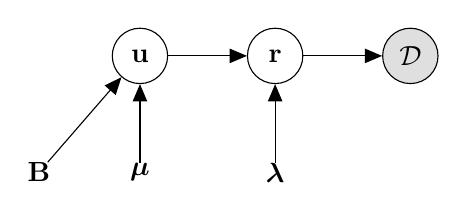
\begin{tikzpicture}
    \node[latent] (u) {$\mathbf{u}$};
    \node[latent, right=of u] (r) {$\mathbf{r}$};
    \node[obs, right=of r] (D) {$\mathcal{D}$};
    \node[const, below=of r] (lambda) {$\bm\lambda$};
    \node[const, below=of u] (mu) {$\bm\mu$};
    \node[const, left=of mu] (B) {$\mathbf{B}$};
    \edge {mu, B} {u};
    \edge {lambda, u} {r};
    \edge {r} {D};
  \end{tikzpicture}
  \caption{Our VI problem expressed as a (simplified)
    Bayesian network. The only observed variable (representing the
    demonstrations) is in a gray circle, modelled latent variables are in white
    circles, and the variational parameters are at the bottom.}
  \label{fig:graphical_model}
\end{figure}

The resulting model is summarised in Figure \ref{fig:graphical_model}. We rely
on $p(\mathcal{D} \mid \mathbf{r})$ as the only link between data and the model.
Since the expression for $q(\mathbf{r} \mid \mathbf{u})$ has both $\mathbf{u}$
and covariance matrices in it, $\mathbf{r}$ depends on both $\mathbf{u}$ and the
parameters of the kernel, $\bm\lambda$. The two remaining dependencies stem from
the fact that the approximating distribution for $\mathbf{u}$ is
$\mathcal{N}(\bm\lambda, \mathbf{BB}^\intercal)$.

As we want to restrict some parameters (namely, $\bm\lambda$ and the diagonal of
$\mathbf{B}$) to positive values, we express them as exponentials and later
adjust their derivatives accordingly. Specifically, we can set $\lambda_i =
e^{\lambda'_i}$ and optimise $\lambda'_i$ using the chain rule:
\[
  \frac{\partial \mathcal{L}}{\partial \lambda'_i} = e^{\lambda'_i}
  \frac{\partial \mathcal{L}}{\partial \lambda_i}.
\]
This way, we restrict $\lambda_i$ to positive values while allowing $\lambda'_i$
to range over $\mathbb{R}$.

Finally, the parameters are initialised as follows:
\begin{alignat*}{3}
  \mu_i &\sim \mathcal{U}(0, 1) \quad &&\text{for } i = 1, \dots, m, \\
  \lambda_0 &\sim \chi^2_5, && \\
  \lambda_i &\sim \chi^2_1 \quad &&\text{for } i = 1, \dots, d, \\
  \diag(\mathbf{B}) &\sim \chi^2_4, && \\
  \text{the rest of } \mathbf{B} &\sim \mathcal{N}(0, 1). &&
\end{alignat*}
The initialisation of $\bm\mu$ mirrors the initialisation of $\mathbf{r}$ in
previous work by Levine et al. \cite{DBLP:conf/nips/LevinePK11}. While they have
constant initial values for $\bm\lambda$, we sample from $\chi^2$ distributions
centred around those values ($5$ for $\lambda_0$ and $1$ for any other
$\lambda_i$). The distributions for initial values of $\mathbf{B}$ are simply
set to provide a reasonable spread of positive values for the diagonal, and both
positive and negative values for all other entries in the matrix.

\subsection{Evidence Lower Bound} \label{sec:elbo}

In this section, we derive and simplify the ELBO for this (now fully specified)
model. Note that in order to keep the derivation simple, we drop all constant
terms in the expression of $\mathcal{L}$, i.e., equality is taken to mean
`equality up to an additive constant'. Also note that all expected values are
with respect to $(\mathbf{u}, \mathbf{r}) \sim q(\mathbf{u}, \mathbf{r})$.

In order to derive the ELBO, let us go back to \eqref{eq:elbo} and
write
\[
  \mathcal{L} = \mathbb{E}[\log\pfull] - \mathbb{E}[\log\approximation].
\]
By substituting in \eqref{eq:full} and \eqref{eq:approximation}, we get
\begin{align*}
  \mathcal{L} &= \mathbb{E}[\log p(\mathbf{u}) + \log p(\mathbf{r} \mid \mathbf{u}) + \log p(\mathcal{D} \mid \mathbf{r})] \\
              &- \mathbb{E}[\log q(\mathbf{u}) + \log q(\mathbf{r} \mid \mathbf{u})].
\end{align*}
Since $q(\mathbf{r} \mid \mathbf{u}) = p(\mathbf{r} \mid \mathbf{u})$, they
cancel each other out. Also notice that
\begin{align*}
  \mathbb{E}[\log p(\mathbf{u}) - \log q(\mathbf{u})] &= -\DKL{q(\mathbf{u})}{p(\mathbf{u})} \\
                                                      &= -\frac{1}{2} (\tr (\Kuu^{-1}\bm\Sigma) + \bm\mu^\intercal\Kuu^{-1}\bm\mu - m \\
                                                      &+ \log |\Kuu| - \log |\bm\Sigma|),
\end{align*}
by the definition of KL divergence between two multivariate Gaussians
\cite{kl}. Hence,
\begin{align*}
  \mathcal{L} &= \mathbb{E}\left[ \sum_{i=1}^N \sum_{t=1}^T Q_{\mathbf{r}}(s_{i,t}, a_{i,t}) - \V(s_{i,t}) \right] \\
              &- \frac{1}{2} \left(\tr \left( \Kuu^{-1}\bm\Sigma \right) + \bm\mu^\intercal\Kuu^{-1}\bm\mu + \log |\Kuu| - \log |\bm\Sigma| \right).
\end{align*}
Using the expressions for $Q_{\mathbf{r}}$ we get
\begin{align*}
  \mathcal{L} &= \mathbb{E}\left[\sum_{i=1}^N \sum_{t=1}^T r(s_{i,t}) - \V(s_{i,t}) + \gamma\sum_{s' \in \mathcal{S}} \mathcal{T}(s_{i,t}, a_{i,t}, s')\V(s') \right] \\
              &- \frac{1}{2} \left(\tr \left( \Kuu^{-1}\bm\Sigma \right) + \bm\mu^\intercal\Kuu^{-1}\bm\mu + \log |\Kuu| - \log |\bm\Sigma| \right).
\end{align*}
We can simplify $\sum_{i=1}^N\sum_{t=1}^Tr(s_{i,t})$ by defining a new vector
$\mathbf{t} = (t_1, \dots, t_{|\mathcal{S}|})^\intercal$, where $t_i$ is the
number of times the state associated with the reward $r_i$ has been visited
across all demonstrations. Then
\begin{align*}
  \mathbb{E} \left[ \sum_{i=1}^N\sum_{t=1}^Tr(s_{i,t}) \right] &= \mathbb{E}[\mathbf{t}^\intercal\mathbf{r}] = \mathbf{t}^\intercal\mathbb{E}[\mathbf{r}] \\
                                                               &= \mathbf{t}^\intercal\mathbb{E}\left[\Kru^\intercal\Kuu^{-1}\mathbf{u}\right] = \mathbf{t}^\intercal\Kru^\intercal\Kuu^{-1}\bm\mu.
\end{align*}
This allows us to simplify $\mathcal{L}$ to
\begin{align*}
  \mathcal{L} &= \mathbf{t}^\intercal\Kru^\intercal\Kuu^{-1}\bm\mu - \mathbb{E}[v] \\
              &- \frac{1}{2} \left(\tr \left( \Kuu^{-1}\bm\Sigma \right) + \bm\mu^\intercal\Kuu^{-1}\bm\mu + \log |\Kuu| - \log |\bm\Sigma| \right),
\end{align*}
where
\[
  v = \sum_{i=1}^N \sum_{t=1}^T \V(s_{i,t}) - \gamma\sum_{s' \in \mathcal{S}}
  \mathcal{T}(s_{i,t}, a_{i,t}, s')\V(s').
\]

\section{Theoretical Justification} \label{sec:proof}

\begin{figure}
  \centering
  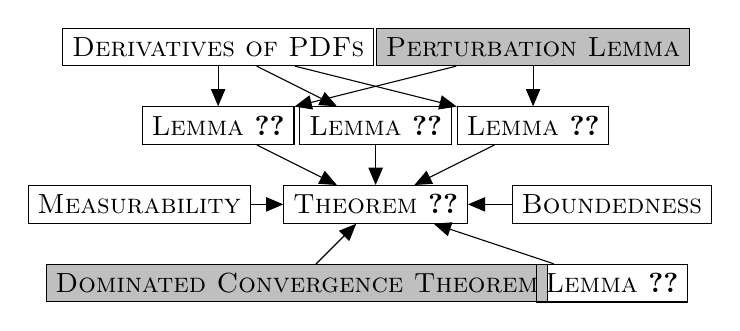
\begin{tikzpicture}
    \node [rectangle, draw, fill=lightgray] (perturbation) at (2, 0) {\textsc{Perturbation Lemma}};
    \node [rectangle, draw, fill=lightgray] (lebesgue) at (-1, -3) {\textsc{Dominated Convergence Theorem}};
    \node [rectangle, draw] (derivatives) at (-2, 0) {\textsc{Derivatives of PDFs}};
    \node [rectangle, draw] (measurability) at (-3, -2) {\textsc{Measurability}};
    \node [rectangle, draw] (boundedness) at (3, -2) {\textsc{Boundedness}};
    \node [rectangle, draw] (lemma1) at (-2, -1) {\textsc{Lemma \ref{lemma:bound1}}};
    \node [rectangle, draw] (lemma2) at (0, -1) {\textsc{Lemma \ref{lemma:bound2}}};
    \node [rectangle, draw] (lemma3) at (2, -1) {\textsc{Lemma \ref{lemma:bound3}}};
    \node [rectangle, draw] (lemma4) at (3, -3) {\textsc{Lemma \ref{lemma:integral_of_r}}};
    \node [rectangle, draw] (theorem) at (0, -2) {\textsc{Theorem \ref{thm:main}}};

    \draw [->] (perturbation) edge (lemma3);
    \draw [->] (perturbation) edge (lemma1);
    \draw [->] (lebesgue) edge (theorem);
    \draw [->] (derivatives) edge (lemma1);
    \draw [->] (derivatives) edge (lemma2);
    \draw [->] (derivatives) edge (lemma3);
    \draw [->] (measurability) edge (theorem);
    \draw [->] (boundedness) edge (theorem);
    \draw [->] (lemma1) edge (theorem);
    \draw [->] (lemma2) edge (theorem);
    \draw [->] (lemma3) edge (theorem);
    \draw [->] (lemma4) edge (theorem);
  \end{tikzpicture}
  \caption{A graphical representation of dependencies between our theoretical
    results. An arrow from $A$ to $B$ means that $A$ was used to prove $B$.
    Results from the literature are in gray.}
  \label{fig:theorems}
\end{figure}

The typical way to optimise a quantity (the ELBO, in this case) involves
computing its gradient. Unfortunately, the term $\mathbb{E}[v]$ in $\mathcal{L}$
complicates the situation. The goal of this section is to show how Theorem
\ref{thm:lebesgue} can be applied to our model in order to derive the gradient
anyway\footnote{This technique is inspired by black box VI
  \cite{DBLP:conf/aistats/RanganathGB14}, but takes a more detailed look at the
  problem and requires significantly more work to prove correctness.}. After
showing that the theorem applies to our situation, we can estimate
$\nabla\mathbb{E}[v]$ with
\begin{align*}
  \nabla\mathbb{E}[v] &= \nabla \iint q(\mathbf{r} \mid \mathbf{u}) q(\mathbf{u})\dx \\
                      &= \iint \nabla[v q(\mathbf{r} \mid \mathbf{u}) q(\mathbf{u})]\dx \\
                      &= \iint \frac{\nabla[v q(\mathbf{r} \mid \mathbf{u})q(\mathbf{u})]}{q(\mathbf{r} \mid \mathbf{u})q(\mathbf{u})} q(\mathbf{r} \mid \mathbf{u}) q(\mathbf{u})\dx \\
                      &\approx \frac{1}{S} \sum_{s=1}^S \frac{\nabla[v q(\mathbf{r}_s \mid \mathbf{u}_s)q(\mathbf{u}_s)]}{q(\mathbf{r}_s \mid \mathbf{u}_s)q(\mathbf{u}_s)},
\end{align*}
which can be computed by drawing $S$ samples $\{(\mathbf{u}_s,
\mathbf{r}_s)\}_{s=1}^S$ from $\approximation$.

Our main goal is Theorem \ref{thm:main}, which allows us to move differentiation
inside the integral. In order to prove it, we use a number of intermediate
results. We start by stating a few derivatives of probability density functions
(PDFs) and covariance matrices, and bound their values with some
easy-to-deal-with polynomials. We then provide a sketch proof of the
measurability of MDP value functions, which is non-obvious due to their
non-trivial definition. Afterwards, we establish bounds for the value functions,
and, after another quick lemma, tackle the main proof of this paper. See Figure
\ref{fig:theorems} for an overview of how these results fit together.

Before that, however, we define a few extra variables in order to simplify
expressions of derivatives:
\begin{align*}
  \mathbf{U} &= (\mathbf{u} - \bm\mu)(\mathbf{u} - \bm\mu)^\intercal, \\
  \mathbf{S} &= \Kru^\intercal\Kuu^{-1}, \\
  \bm\Gamma &= \Krr - \mathbf{S}\Kru, \\
  \mathbf{R} &= \mathbf{S}\frac{\partial \Kru}{\partial \lambda_i} - \frac{\partial \Krr}{\partial \lambda_i} + \left( \frac{\partial \Kru^\intercal}{\partial \lambda_i} - \mathbf{S}\frac{\partial \Kuu}{\partial \lambda_i} \right) \Kuu^{-1}\Kru, \\
  Q &= (\mathbf{u} - \bm\mu)^\intercal\bm\Sigma^{-1}(\mathbf{u} - \bm\mu).
\end{align*}
Also note that throughout this section the word `constant' means `constant with
respect to $\mathbf{u}$ and $\mathbf{r}$'.

\begin{restatable}[Derivatives of PDFs]{lemma}{derivatives} \label{lemma:derivatives}
  \leavevmode
  \begin{enumerate}
  \item $\frac{\partial q(\mathbf{u})}{\partial \bm\mu} =
    \frac{1}{2}q(\mathbf{u})(\bm\Sigma^{-1} + \bm\Sigma^{-\intercal})(\mathbf{u}
    - \bm\mu)$.
  \item
    \begin{enumerate}
    \item
      $\frac{\partial q(\mathbf{u})}{\partial \bm\Sigma} =
      \frac{1}{2}q(\mathbf{u})(\bm\Sigma^{-1}\mathbf{U}\bm\Sigma^{-1} -
      \bm\Sigma^{-1})$.
    \item
      $\frac{\partial q(\mathbf{u})}{\partial \mathbf{B}} =
      q(\mathbf{u})(\bm\Sigma^{-1}\mathbf{U}\bm\Sigma^{-1} -
      \bm\Sigma^{-1})\mathbf{B}$.
    \end{enumerate}
  \item For $i = 0, \dots, d$,
    \begin{enumerate}
    \item
      \begin{align*}
        \frac{\partial q(\mathbf{r} \mid \mathbf{u})}{\partial \lambda_i} &= \frac{1}{2}q(\mathbf{r} \mid \mathbf{u}) (|\bm\Gamma|^{-1} \tr(\mathbf{R} \adj(\bm\Gamma)) \\
                                                                          &- (\mathbf{r} - \mathbf{Su})^\intercal\bm\Gamma^{-1}\mathbf{R}\bm\Gamma^{-1}(\mathbf{r} - \mathbf{Su})).
      \end{align*}
    \item For any covariance matrix $\mathbf{K}$,
      \[
        \frac{\partial \mathbf{K}}{\partial \lambda_i} =
        \begin{cases}
          \frac{1}{\lambda_i}\mathbf{K} & \text{if } i = 0, \\
          \mathbf{L} & \text{otherwise,}
        \end{cases}
      \]
      where
      \[
        L_{j,k} = k(\mathbf{x}_j, \mathbf{x}_k) \left( -\frac{1}{2}(x_{j,i} -
          x_{k,i})^2 - \mathbbm{1}[j \ne k]\sigma^2 \right).
      \]
    \end{enumerate}
  \end{enumerate}
\end{restatable}

% TODO: need some editing
\begin{lemma} \label{lemma:bound1}
  Let $i \in \{ 0, \dots, d \}$ and $\epsilon > 0$ be arbitrary. Furthermore,
  let $c : \mathbb{R}^{|\mathcal{S}|} \times \mathbb{R}^m \to (\lambda_i -
  \epsilon, \lambda_i + \epsilon) \subset \mathbb{R}$ be a function with a
  codomain arbitrarily close to $\lambda_i$. Then
  \[
    \left. \frac{\partial q(\mathbf{r} \mid \mathbf{u})}{\partial \lambda_i}
    \right|_{\lambda_i = c(\mathbf{r}, \mathbf{u})}
  \]
  has upper and lower bounds of the form $q(\mathbf{r} \mid
  \mathbf{u})d(\mathbf{u})$, where $d(\mathbf{u}) \in \mathbb{R}_2[\mathbf{u}]$.
\end{lemma}
\begin{proof}
  Remember that
  \begin{align*}
    \frac{\partial q(\mathbf{r} \mid \mathbf{u})}{\partial \lambda_i} &= \frac{1}{2}q(\mathbf{r} \mid \mathbf{u}) (|\bm\Gamma|^{-1} \tr(\mathbf{R} \adj(\bm\Gamma)) \\
                                                                      &- (\mathbf{r} - \mathbf{Su})^\intercal\bm\Gamma^{-1}\mathbf{R}\bm\Gamma^{-1}(\mathbf{r} - \mathbf{Su})).
  \end{align*}
  by Lemma \ref{lemma:derivatives}. Let $\mathbf{K}$ be any covariance
  matrix and
  \[
    \mathbf{A} = \frac{1}{\lambda_0} \mathbf{K}.
  \]

  First, we will show that
  \[
    \mathbf{K}|_{\lambda_i = c(\mathbf{r}, \mathbf{u})} \to 0 \quad \text{and}
    \quad \left. \frac{\mathbf{\partial K}}{\partial \lambda_i}
    \right|_{\lambda_i = c(\mathbf{r}, \mathbf{u})} \to 0
  \]
  as $\epsilon \to 0$.
  We can easily establish constant upper and lower bounds on
  $\mathbf{K}|_{\lambda_i = c(\mathbf{r}, \mathbf{u})}$ by the boundedness of
  $c$ and continuity of the covariance function. Similar reasoning combined with
  the expressions for derivatives of covariance matrices in Lemma
  \ref{lemma:derivatives} gives constant upper and lower bounds on the elements
  of
  \[
    \left. \frac{\mathbf{\partial K}}{\partial \lambda_i} \right|_{\lambda_i =
      c(\mathbf{r}, \mathbf{u})}
  \]
  as well.

  % Inverse of a covariance matrix
  Now, we will show that $\mathbf{K}^{-1}|_{\lambda_i = c(\mathbf{r},
    \mathbf{u})}$ exists and
  \[
    \lim_{\epsilon \to 0} \mathbf{K}^{-1}|_{\lambda_i = c(\mathbf{r},
      \mathbf{u})} = \mathbf{K}.
  \]
  If $i = 0$, then $\mathbf{K}|_{\lambda_i = c(\mathbf{r}, \mathbf{u})} =
  c(\mathbf{r}, \mathbf{u})\mathbf{A}$. Therefore\footnote{Note that since
    $\lambda_0 \ne 0$, $c(\mathbf{r}, \mathbf{u}) \ne 0$ for small enough
    $\epsilon$.},
  \begin{align*}
    \mathbf{K}^{-1}|_{\lambda_i = c(\mathbf{r}, \mathbf{u})} &=
                                                               \frac{1}{c(\mathbf{r}, \mathbf{u})}\mathbf{A}^{-1} \\
                                                             &\to \frac{1}{\lambda_0}\mathbf{A}^{-1} = \frac{1}{\lambda_0} \left( \frac{1}{\lambda_0}\mathbf{K} \right)^{-1} = \mathbf{K}^{-1}
  \end{align*}
  as $\epsilon \to 0$.

  We will now show the same result for $\lambda_i > 0$. Let
  \[
    S = \sum_{n \in \{ 1, \dots, d \} \setminus \{ i \}} \frac{\lambda_n}{2}
    (x_{j,n} - x_{k,n})^2 + \mathbbm{1}[j \ne k]\sigma^2 \lambda_n
  \]
  and $\delta = c(\mathbf{r}, \mathbf{u}) - \lambda_i$ so that $c(\mathbf{r},
  \mathbf{u}) = \lambda_i + \delta$, and $\lim_{\epsilon \to 0} \delta = 0$.
  Then,
  \begin{align*}
    &k(\mathbf{x}_j, \mathbf{x}_k)|_{\lambda_i = c(\mathbf{r}, \mathbf{u})} = \!\begin{multlined}[t]
      \lambda_0 \exp \left( \vphantom{\frac{1}{2}} \right. -\frac{1}{2} c(\mathbf{r}, \mathbf{u})(x_{j,i} - x_{k,i})^2\\
      - \mathbbm{1}[j \ne k]\sigma^2c(\mathbf{r}, \mathbf{u}) - S \left. \vphantom{\frac{1}{2}} \right)
    \end{multlined} \\
    &= \!\begin{multlined}[t]
      \lambda_0 \exp \left( \vphantom{\frac{1}{2}} \right. -\frac{1}{2} (\lambda_i + \delta)(x_{j,i} - x_{k,i})^2 \\
      - \mathbbm{1}[j \ne k]\sigma^2(\lambda_i + \delta) - S \left. \vphantom{\frac{1}{2}} \right)
    \end{multlined} \\
    &= \!\begin{multlined}[t]
      \lambda_0 \exp \left( \vphantom{\frac{1}{2}} \right. -\frac{1}{2}(\mathbf{x}_j - \mathbf{x}_k)^\intercal \bm\Lambda (\mathbf{x}_j - \mathbf{x}_k) - \mathbbm{1}[j \ne k]\sigma^2\tr(\bm\Lambda) \\
      - \frac{\delta}{2}(x_{j,i} - x_{k,i})^2 - \mathbbm{1}[j \ne k]\sigma^2\delta \left. \vphantom{\frac{1}{2}} \right)
    \end{multlined} \\
    &= k(\mathbf{x}_j, \mathbf{x}_k)\exp \left( \vphantom{\frac{1}{2}} \right. -\frac{\delta}{2}(x_{j,i} - x_{k,i})^2 - \mathbbm{1}[j \ne k]\sigma^2\delta \left. \vphantom{\frac{1}{2}} \right) \\
    &= \!\begin{multlined}[t]
      k(\mathbf{x}_j, \mathbf{x}_k) + k(\mathbf{x}_j, \mathbf{x}_k) \left( \exp
        \left( -\frac{\delta}{2}(x_{j,i} - x_{k,i})^2 \right. \right. \\
      -\mathbbm{1}[j \ne k]\sigma^2\delta \left. \left. \vphantom{\frac{1}{2}} \right) - 1 \right)
    \end{multlined}
  \end{align*}
  Hence, we can express $\mathbf{K}|_{\lambda_i = c(\mathbf{r}, \mathbf{u})}$ as
  $\mathbf{K}|_{\lambda_i = c(\mathbf{r}, \mathbf{u})} = \mathbf{K} +
  \mathbf{E}$, where $\mathbf{E}$ is defined as
  \[
    E_{j,k} = k(\mathbf{x}_j, \mathbf{x}_k) \left( \exp \left(
        -\frac{\delta}{2}(x_{j,i} - x_{k,i})^2 \right. \right. -\mathbbm{1}[j
    \ne k]\sigma^2\delta \left. \left. \vphantom{\frac{1}{2}} \right) - 1
    \right).
  \]
  By this definition,
  \[
    \lim_{\epsilon \to 0} E_{j,k} = 0.
  \]
  Then, since $\mathbf{K}$ is invertible, Lemma \ref{lemma:perturbation} shows
  the existence of $\mathbf{K}^{-1}_{\lambda_i = c(\mathbf{r}, \mathbf{u})}$ and
  gives upper and lower bounds on all of its elements.

  This is enough to prove constant upper and lower bounds on
  $\mathbf{S}$, $\bm\Gamma$, and $\mathbf{R}$ (all with $\lambda_i$ replaced
  with $c(\mathbf{r}, \mathbf{u})$), which means that $(\mathbf{r} -
  \mathbf{Su})^\intercal\bm\Gamma^{-1}\mathbf{R}\bm\Gamma^{-1}(\mathbf{r} -
  \mathbf{Su})|_{\lambda_i = c(\mathbf{r}, \mathbf{u})}$ has upper and lower
  bounds in $\mathbb{R}_2[\mathbf{u}]$.
  
  Since
  \[
    \lim_{\epsilon \to 0} \bm\Gamma|_{\lambda_i = c(\mathbf{r}, \mathbf{u})} =
    \bm\Gamma,
  \]
  we also have that
  \[
    \lim_{\epsilon \to 0} \det(\bm\Gamma)|_{\lambda_i = c(\mathbf{r}, \mathbf{u})} =
    \det(\bm\Gamma).
  \]
  Assuming that
  $\bm\Gamma$ is invertible so that $q(\mathbf{r} \mid \mathbf{u})$ exists,
  \[
    \det(\bm\Gamma)|_{\lambda_i = c(\mathbf{r}, \mathbf{u})} \ne 0
  \]
  for small enough $\epsilon$, and, thus, $\det(\bm\Gamma)^{-1}|_{\lambda_i =
    c(\mathbf{r}, \mathbf{u})}$ exists and has constant bounds.

  Recall that
  \[
    \bm\Gamma = \Krr - \mathbf{S}\Kru = \Krr - \Kru^\intercal\Kuu^{-1}\Kru.
  \]
  We have already demonstrated that for $\mathbf{K} \in \{ \Krr, \Kru, \Kuu^{-1}
  \}$,
  \[
    \lim_{\epsilon \to 0}\mathbf{K}|_{\lambda_i = c(\mathbf{r}, \mathbf{u})} =
    \mathbf{K}.
  \]
  We can use a general fact that if $\lim_{x \to 0} f(x) = f$,
  then $f(x) = f + g(x)$ for some function $g$ such that $\lim_{x \to 0} g(x) =
  0$ to define matrices $\Err$, $\Eru$, and $\Euu$ such that
  \begin{alignat*}{3}
    \Krr|_{\lambda_i = c(\mathbf{r}, \mathbf{u})} &= \Krr + \Err, &&\Err \to
    \mathbf{O}_{|\mathcal{S}|}, \\
    \Kru|_{\lambda_i = c(\mathbf{r}, \mathbf{u})} &= \Kru + \Eru, \quad
    \text{and} \quad &&\Eru \to \mathbf{O}_{|\mathcal{S}|, m}, \\
    \Kuu^{-1}|_{\lambda_i = c(\mathbf{r}, \mathbf{u})} &= \Kuu^{-1} + \Euu,
    &&\Euu \to \mathbf{O}_{m}.
  \end{alignat*}
  as $\epsilon \to 0$. Then, $\bm\Gamma|_{\lambda_i = c(\mathbf{r}, \mathbf{u})}
  = \bm\Gamma + \mathbf{E}$, where
  \begin{align*}
    \mathbf{E} &= \Err - \Kru^\intercal\Kuu^{-1}\Eru - \Kru^\intercal\Euu(\Kru + \Eru) \\
               &- \Eru^\intercal(\Kuu^{-1} + \Euu)(\Kru + \Eru) \\
               &\to \mathbf{O}_{|\mathcal{S}|}
  \end{align*}
  as $\epsilon \to 0$. Thus, Lemma \ref{lemma:perturbation} shows that
  $\bm\Gamma^{-1}|_{\lambda_i = c(\mathbf{r}, \mathbf{u})}$ exists and provides
  constant bounds on its elements.

  Since we already know that $\bm\Gamma^{-1}|_{\lambda_i = c(\mathbf{r},
    \mathbf{u})}$ and $\det(\bm\Gamma)|_{\lambda_i = c(\mathbf{r}, \mathbf{u})}$
  are bounded, so is $\adj(\bm\Gamma) =
  \det(\bm\Gamma)\bm\Gamma^{-1}|_{\lambda_i = c(\mathbf{r}, \mathbf{u})}$. Thus,
  we have constant bounds on
  $|\bm\Gamma|^{-1}\tr(\mathbf{R}\adj(\bm\Gamma))|_{\lambda_i = c(\mathbf{r},
    \mathbf{u})}$, which means that
  \[
    \left. \frac{\partial q(\mathbf{r} \mid \mathbf{u})}{\partial \lambda_i}
    \right|_{\lambda_i = c(\mathbf{r}, \mathbf{u})}
  \]
  has the required bounds.
\end{proof}
% TOOD: epsilon should not be treated as a constant. Revise the whole theory
% section.

\begin{remark}
  In order to find a derivative such as $\frac{\partial q(\mathbf{u})}{\partial
    \mu_i}$, we can find $\frac{\partial q(\mathbf{u})}{\partial \bm\mu}$ and
  simply take the $i$th element. A similar line of reasoning applies to matrices
  as well. Thus, we only need to consider derivatives with respect to $\bm\mu$
  and $\bm\Sigma$.
\end{remark}

\begin{lemma} \label{lemma:bound2}
  Let $c : \mathbb{R}^{|\mathcal{S}|} \times \mathbb{R}^m \to (a, b) \subset
  \mathbb{R}$ be an arbitrary bounded function. Then, for $i = 1, \dots, m$,
  every element of
  \[
    \left. \frac{\partial q(\mathbf{u})}{\partial \bm\mu} \right|_{\mu_i =
      c(\mathbf{r}, \mathbf{u})}
  \]
  has upper and lower bounds of the form $q(\mathbf{u})d(\mathbf{u})$,
  where $d(\mathbf{u}) \in \mathbb{R}_1[\mathbf{u}]$.
\end{lemma}
\begin{proof}
  Using Lemma \ref{lemma:derivatives},
  \[
    \left. \frac{\partial q(\mathbf{u})}{\partial \bm\mu} \right|_{\mu_i =
      c(\mathbf{r}, \mathbf{u})} = \frac{1}{2}q(\mathbf{u})(\bm\Sigma^{-1} +
    \bm\Sigma^{-\intercal})(\mathbf{u} - \mathbf{c}(\mathbf{r}, \mathbf{u})),
  \]
  where $\mathbf{c}(\mathbf{r}, \mathbf{u}) = (\mu_1, \dots, \mu_{i - 1},
  c(\mathbf{r}, \mathbf{u}), \mu_{i + 1} \dots, \mu_m)^\intercal$. Since
  $c(\mathbf{r}, \mathbf{u})$ is bounded and $\bm\Sigma^{-1} +
  \bm\Sigma^{-\intercal}$ is a constant matrix, we can use the bounds on
  $c(\mathbf{r}, \mathbf{u})$ to manufacture both upper and lower bounds on
  \[
     \left. \frac{\partial q(\mathbf{u})}{\partial \bm\mu} \right|_{\mu_i =
      c(\mathbf{r}, \mathbf{u})}
  \]
  of the required form.
\end{proof}

\begin{lemma} \label{lemma:bound3}
  Let $i, j = 1, \dots, m$, and let $\epsilon > 0$ be arbitrary. Furthermore,
  let
  \[
    c : \mathbb{R}^{|\mathcal{S}|} \times \mathbb{R}^m \to (\Sigma_{i,j} - \epsilon,
    \Sigma_{i,j} + \epsilon) \subset \mathbb{R}
  \]
  be a function with a codomain arbitrarily close to $\Sigma_{i,j}$. Then every
  element of
  \[
    \left. \frac{\partial q(\mathbf{u})}{\partial \bm\Sigma} \right|_{\Sigma_{i,j} =
    c(\mathbf{r}, \mathbf{u})}
  \]
  has upper and lower bounds of the form $q(\mathbf{u})d(\mathbf{u})$, where
  $d(\mathbf{u}) \in \mathbb{R}_2[\mathbf{u}]$.
\end{lemma}
\begin{proof}
  Using Lemma \ref{lemma:derivatives},
  \[
    \left. \frac{\partial q(\mathbf{u})}{\partial \bm\Sigma} \right|_{\Sigma_{i,j} =
    c(\mathbf{r}, \mathbf{u})} =
    \frac{1}{2}q(\mathbf{u})(\mathbf{C}(\mathbf{r},
    \mathbf{u})^{-\intercal}\mathbf{UC}(\mathbf{r}, \mathbf{u})^{-\intercal} -
    \mathbf{C}(\mathbf{r}, \mathbf{u})^{-\intercal}),
  \]
  where
  \[
    [\mathbf{C}(\mathbf{r}, \mathbf{u})]_{k,l} =
    \begin{cases}
      c(\mathbf{r}, \mathbf{u}) & \text{if } (k, l) = (i, j), \\
      \Sigma_{k,l} & \text{otherwise.}
    \end{cases}
  \]
  We can also express $\mathbf{C}(\mathbf{r},\mathbf{u})$ as
  $\mathbf{C}(\mathbf{r}, \mathbf{u}) = \bm\Sigma + \mathbf{E}(\mathbf{r},
  \mathbf{u})$, where
  \[
    [\mathbf{E}(\mathbf{r}, \mathbf{u})]_{k,l} =
    \begin{cases}
      c(\mathbf{r}, \mathbf{u}) - \Sigma_{i,j} & \text{if } (k, l) = (i, j), \\
      0 & \text{otherwise.}
    \end{cases}
  \]
  We begin by establishing upper and lower bounds on $\mathbf{C}(\mathbf{r},
  \mathbf{u})^{-1}$. For this, we use the maximum norm $\lVert \cdot
  \rVert_\infty$ on both vectors and matrices. We can apply Lemma
  \ref{lemma:perturbation} to $\bm\Sigma$ and $\mathbf{E}(\mathbf{r},
  \mathbf{u})$ since
  \[
    \lVert \mathbf{E}(\mathbf{r}, \mathbf{u}) \rVert_\infty = \max_k \sum_l
    |[\mathbf{E}(\mathbf{r}, \mathbf{u})]_{k,l}| = |c(\mathbf{r}, \mathbf{u}) -
    \Sigma_{i,j}| < \epsilon
  \]
  can be made arbitrarily small so that $\lVert \bm\Sigma^{-1} \rVert_\infty
  \lVert \mathbf{E}(\mathbf{r}, \mathbf{u}) \rVert_\infty < 1$. Then
  $\mathbf{C}(\mathbf{r}, \mathbf{u})$ is invertible, and
  \[
    \lVert \mathbf{C}(\mathbf{r}, \mathbf{u})^{-1} \rVert_\infty \le
    \frac{\lVert \bm\Sigma^{-1} \rVert_\infty}{1 - \lVert \bm\Sigma^{-1}
      \rVert_\infty \lVert \mathbf{E}(\mathbf{r}, \mathbf{u}) \rVert_\infty} <
    \frac{\lVert \bm\Sigma^{-1} \rVert_\infty}{1 - \lVert \bm\Sigma^{-1}
      \rVert_\infty \epsilon},
  \]
  which means that
  \[
    \max_k \sum_l \left| [\mathbf{C}(\mathbf{r}, \mathbf{u})^{-1}]_{k,l} \right|
    < \frac{\lVert \bm\Sigma^{-1} \rVert_\infty}{1 - \lVert \bm\Sigma^{-1}
      \rVert_\infty \epsilon},
  \]
  i.e., for any row $k$ and column $l$,
  \[
    \left| [\mathbf{C}(\mathbf{r}, \mathbf{u})^{-1}]_{k,l} \right| <
    \frac{\lVert \bm\Sigma^{-1} \rVert_\infty}{1 - \lVert \bm\Sigma^{-1}
      \rVert_\infty \epsilon},
  \]
  which bounds all elements of $\mathbf{C}(\mathbf{r}, \mathbf{u})^{-1}$ as
  required. Since every element of $\mathbf{U} = (\mathbf{u} - \bm\mu)(\mathbf{u} -
  \bm\mu)^\intercal$ is in $\mathbb{R}_2[\mathbf{u}]$, and the elements of
  $\mathbf{C}(\mathbf{r}, \mathbf{u})^{-1}$ are bounded, the desired result
  follows.
\end{proof}

\begin{remark}
  MDP values are characterised by both a state and a reward function/vector. In
  this section, we think of the value function as $V : \mathcal{S} \to
  \mathbb{R}^{|\mathcal{S}|} \to \mathbb{R}$, i.e., $V$ takes a state $s \in
  \mathcal{S}$ and returns a function $V(s) : \mathbb{R}^{|\mathcal{S}|} \to
  \mathbb{R}$ that takes a reward vector $\mathbf{r} \in
  \mathbb{R}^{|\mathcal{S}|}$ and returns a value of the state $s$, $\V(s) \in
  \mathbb{R}$. Given a reward vector, the function $V(s)$ computes the values of
  all states and returns the value of state $s$.
\end{remark}

\begin{proposition}[Measurability] \label{thm:measurability}
  MDP value functions $V(s) : \mathbb{R}^{|\mathcal{S}|} \to \mathbb{R}$ (for $s
  \in \mathcal{S}$) are Lebesgue measurable.
\end{proposition}
\begin{proof}
  For any reward vector $\mathbf{r} \in \mathbb{R}^{|\mathcal{S}|}$, the
  collection of converged value functions $\{ \V(s) \mid s \in
  \mathcal{S} \}$ satisfy
  \begin{equation} \label{eq:linear_mdp}
    \V(s) = \log \sum_{a \in \mathcal{A}}
    \exp\left( r(s) + \gamma\sum_{s' \in \mathcal{S}} \mathcal{T}(s, a,
      s')\V(s') \right)
  \end{equation}
  for all $s \in \mathcal{S}$. Let $s_0 \in \mathcal{S}$ be an arbitrary state.
  In order to prove that $V(s_0)$ is measurable, it is enough to show that for
  any $\alpha \in \mathbb{R}$, the set
  \[
    \left\{ \mathbf{r} \in \mathbb{R}^{|\mathcal{S}|} \; \middle|
    \begin{aligned}
      \;&\V(s_0) \in (-\infty, \alpha); \\
      \;&\V(s) \in \mathbb{R} \text{ for all } s \in \mathcal{S} \setminus \{ s_0 \}; \\
      \;&\text{\eqref{eq:linear_mdp} is satisfied by all } s \in
      \mathcal{S}
    \end{aligned}
    \right\}
  \]
  is measurable. Since this set can be constructed in Zermelo-Fraenkel set
  theory \emph{without} the axiom of choice, it is measurable
  \cite{herrlich2006axiom}, which proves that $V(s)$ is a measurable function
  for any $s \in \mathcal{S}$.
\end{proof}

\begin{proposition}[Boundedness] \label{thm:bound}
  If the initial values of the MDP value function satisfy the following
  bound, then the bound remains satisfied throughout value iteration:
  \begin{equation} \label{eq:bound}
    |\V(s)| \le \vbound.
  \end{equation}
\end{proposition}
\begin{proof}
  We begin by considering \eqref{eq:bound} without taking the absolute value of
  $\V(s)$, i.e.,
  \begin{equation} \label{eq:positive_bound}
    \V(s) \le \vbound,
  \end{equation}
  and assuming that the initial values of $\{ \V(s) \mid s \in \mathcal{S} \}$
  already satisfy \eqref{eq:positive_bound}. Recall that for each $s \in
  \mathcal{S}$, the value of $\V(s)$ is updated by applying
  \eqref{eq:update_rule}. Note that both $\log$ and $\exp$ are increasing
  functions, $\gamma > 0$, and the $\mathcal{T}$ function gives a probability (a
  non-negative number). Thus
  \begin{align*}
    \V(s) &\le \log \sum_{a \in \mathcal{A}} \exp\left( r(s) + \gamma\sum_{s' \in \mathcal{S}} \mathcal{T}(s, a, s')\frac{\rinf + \log|\mathcal{A}|}{1 - \gamma} \right) \\
          &= \log \sum_{a \in \mathcal{A}} \exp\left( r(s) + \frac{\gamma (\rinf + \log|\mathcal{A}|)}{1 - \gamma}\sum_{s' \in \mathcal{S}} \mathcal{T}(s, a, s') \right) \\
          &= \log \sum_{a \in \mathcal{A}} \exp\left( r(s) + \frac{\gamma (\rinf + \log|\mathcal{A}|)}{1 - \gamma} \right)
  \end{align*}
  by the definition of $\mathcal{T}$. Then
  \begin{align*}
    \V(s) &\le \log \left( |\mathcal{A}| \exp\left( r(s) + \frac{\gamma (\rinf + \log|\mathcal{A}|)}{1 - \gamma} \right) \right) \\
          &= \log \left( \exp\left( \log|\mathcal{A}| + r(s) + \frac{\gamma (\rinf + \log|\mathcal{A}|)}{1 - \gamma} \right) \right) \\
          &= \log|\mathcal{A}| + r(s) + \frac{\gamma (\rinf + \log|\mathcal{A}|)}{1 - \gamma} \\
          &= \frac{\gamma (\rinf + \log|\mathcal{A}|) + (1 - \gamma)(\log|\mathcal{A}| + r(s))}{1 - \gamma} \\
          &\le \frac{\gamma (\rinf + \log|\mathcal{A}|) + (1 - \gamma)(\log|\mathcal{A}| + \rinf)}{1 - \gamma} \\
          &= \vbound
  \end{align*}
  by the definition of $\rinf$.

  The proof for
  \begin{equation} \label{eq:negative_bound}
    \V(s) \ge \frac{\rinf + \log|\mathcal{A}|}{\gamma - 1}
  \end{equation}
  follows the same argument until we get to
  \begin{align*}
    \V(s) &\ge \frac{\gamma(\rinf + \log|\mathcal{A}|) + (\gamma - 1)(\log|\mathcal{A}| + r(s))}{\gamma - 1} \\
          &\ge \frac{\gamma(\rinf + \log|\mathcal{A}|) + (\gamma - 1)(-\log|\mathcal{A}| -\rinf)}{\gamma - 1} \\
          &= \frac{\rinf + \log|\mathcal{A}|}{\gamma - 1},
  \end{align*}
  where we use the fact that $r(s) \ge -\rinf - 2\log|\mathcal{A}|$. Combining
  \eqref{eq:positive_bound} and \eqref{eq:negative_bound} gives
  \eqref{eq:bound}.
\end{proof}

\begin{lemma} \label{lemma:integral_of_r}
  \[
    \int \lVert \mathbf{r} \rVert_\infty q(\mathbf{r} \mid \mathbf{u})\,d\mathbf{r} \le a +
    \lVert \Kru^\intercal \Kuu^{-1} \mathbf{u} \rVert_1,
  \]
  where $a$ is a constant independent of $\mathbf{u}$.
\end{lemma}
\begin{proof}
  Since $\rinf \le \lVert \mathbf{r} \rVert_1$,
  \[
    \int \lVert \mathbf{r} \rVert_\infty q(\mathbf{r} \mid \mathbf{u})\,d\mathbf{r} \le \int
    \lVert \mathbf{r} \rVert_1 q(\mathbf{r} \mid \mathbf{u})\,d\mathbf{r} =
    \sum_{i=1}^{|\mathcal{S}|} \mathbb{E}[|r_i|].
  \]
  As each $\mathbb{E}[|r_i|]$ is a mean of a folded Gaussian distribution,
  \[
    \mathbb{E}[|r_i|] = \sigma_i \sqrt{\frac{2}{\pi}} \exp
    \left(-\frac{\xi_i^2}{2\sigma_i^2} \right) + \xi_i \left( 1 - 2\Phi \left(
        -\frac{\xi_1}{\sigma_1} \right) \right),
  \]
  where $\xi_i = \left[\Kru^\intercal\Kuu^{-1}\mathbf{u}\right]_i$, $\sigma_i =
  \sqrt{[\Krr - \Kru^\intercal\Kuu^{-1}\Kru]_{i,i}}$\footnote{The expression
    under the square root sign is non-negative because $\Krr -
    \Kru^\intercal\Kuu^{-1}\Kru$ is a covariance matrix of a Gaussian
    distribution, hence also positive semi-definite, which means that its
    diagonal entries are non-negative.}, and $\Phi$ is the cumulative
  distribution function of the standard Gaussian. Furthermore,
  \[
    \mathbb{E}[|r_i|] \le \sigma_i\sqrt{\frac{2}{\pi}} + |\xi_i|,
  \]
  as $\sigma_i$ is non-negative, and $\Phi(x) \in [0, 1]$ for all $x$. Since
  \[ \sum_{i=1}^{|\mathcal{S}|} |\xi_i| = \lVert \Kru^\intercal \Kuu^{-1}
    \mathbf{u} \rVert_1, \]
  we can set
  \[ a = \sum_{i=1}^{|\mathcal{S}|} \sigma_i \sqrt{\frac{2}{\pi}} \]
  to get the desired result.
\end{proof}

Our main theorem is a specialised version of an integral differentiation result
by Timoney \cite{lecture_notes}.
\begin{theorem} \label{thm:main}
  Whenever the derivative exists,
  \[
    \dt\iint
    \V(s)q(\mathbf{r} \mid \mathbf{u})q(\mathbf{u})\dx
    = \iint
    \dt[\V(s)q(\mathbf{r} \mid \mathbf{u})q(\mathbf{u})]\dx,
  \]
  where $t$ is any scalar part of $\bm\mu$, $\bm\Sigma$, or $\bm\lambda$.
\end{theorem}
\begin{proof}
  Let
  \begin{align*}
    \f &= \V(s)q(\mathbf{r} \mid \mathbf{u})q(\mathbf{u}), \\
    F(t) &= \iint \f\dx,
  \end{align*}
  and fix the value of $t$. Let $(t_n)_{n=1}^\infty$ be any sequence such that
  $\lim_{n \to \infty} t_n = t$, but $t_n \ne t$ for all $n$. We want to show
  that
  \begin{equation} \label{eq:to_prove}
    F'(t) = \lim_{n \to \infty} \frac{F(t_n) - F(t)}{t_n - t} = \iint \df\dx.
  \end{equation}
  We have
  \[
    \begin{split}
      \frac{F(t_n) - F(t)}{t_n - t} &= \iint \frac{\ftn - \f}{t_n - t}\dx \\
      &= \iint \fn\dx,
    \end{split}
  \]
  where
  \[
    \fn = \frac{\ftn - \f}{t_n - t}.
  \]
  Since
  \[
    \lim_{n \to \infty} \fn = \df,
  \]
  \eqref{eq:to_prove} follows from Theorem \ref{thm:lebesgue} as soon as we show
  that both $f$ and $f_n$ are measurable and find a non-negative integrable
  function $g$ such that for all $n$, $\mathbf{r}$, $\mathbf{u}$,
  \[
    |\fn| \le \g.
  \]
  The MDP value function is measurable by Proposition \ref{thm:measurability}.
  The result of multiplying or adding measurable functions (e.g., probability
  density functions) to a measurable function is still measurable. Thus,
  both $f$ and $f_n$ are measurable.

  It remains to find $g$. For notational simplicity and without loss of
  generality, we will temporarily assume that $t$ is a parameter of
  $q(\mathbf{r} \mid \mathbf{u})$. Then
  \[
    |\fn| = |\V(s)| \left| \frac{q(\mathbf{r} \mid \mathbf{u})|_{t =
          t_n} - q(\mathbf{r} \mid \mathbf{u})}{t_n - t} \right| q(\mathbf{u})
  \]
  since PDFs are non-negative. An upper bound for
  $|\V(s)|$ is given by Proposition \ref{thm:bound}, while
  \[
    \frac{q(\mathbf{r} \mid \mathbf{u})|_{t = t_n} - q(\mathbf{r} \mid \mathbf{u})}{t_n - t} = \left.
      \frac{\partial q(\mathbf{r} \mid \mathbf{u})}{\partial t} \right|_{t = c(\mathbf{r},
      \mathbf{u})}
  \]
  for some function $c : \mathbb{R}^{|\mathcal{S}|} \times \mathbb{R}^m \to
  (\min\{t, t_n\}, \max\{t, t_n\})$ due to the mean value theorem (since $q$ is
  a continuous and differentiable function of $t$, regardless of the specific
  choices of $q$ and $t$).

  We then have that
  \[
    |\fn| \le \vbound \left| \left. \frac{\partial
          q(\mathbf{r} \mid \mathbf{u})}{\partial t} \right|_{t=c(\mathbf{r}, \mathbf{u})}
    \right| q(\mathbf{u}).
  \]
  The bound is clearly non-negative and measurable. It remains to show that it
  is also integrable. Depending on what $t$ represents, we can use one of the
  Lemmas \ref{lemma:bound1}, \ref{lemma:bound2}, and \ref{lemma:bound3}, which
  gives us two polynomials $p_1(\mathbf{u}), p_2(\mathbf{u}) \in
  \mathbb{R}_2[\mathbf{u}]$ such that
  \[
    p_1(\mathbf{u})q(\mathbf{r} \mid \mathbf{u}) < \left. \frac{\partial q(\mathbf{r} \mid \mathbf{u})}{\partial
        t} \right|_{t=c(\mathbf{r}, \mathbf{u})} < p_2(\mathbf{u})q(\mathbf{r} \mid \mathbf{u}).
  \]
  Then
  \[
    \left| \left. \frac{\partial q(\mathbf{r} \mid \mathbf{u})}{\partial t}
      \right|_{t=c(\mathbf{r}, \mathbf{u})} \right| < q(\mathbf{r} \mid \mathbf{u}) \max \{
    |p_1(\mathbf{u})|, |p_2(\mathbf{u})| \}.
  \]
  We can now apply Lemma \ref{lemma:integral_of_r}, which allows us to integrate
  out $\mathbf{r}$, and we are left with showing the existence of
  \begin{equation} \label{eq:remaining_integral}
    \int \left( a + \lVert \Kru^\intercal \Kuu^{-1} \mathbf{u} \rVert_1 \right) \max \{|p_1(\mathbf{u})|, |p_2(\mathbf{u})| \} q(\mathbf{u})\,d\mathbf{u},
  \end{equation}
  where $a$ is a constant. The integral
  \[
    \int \max \left\{
      \begin{aligned}
        &|p_1(\mathbf{u})|, \\
        &|p_2(\mathbf{u})|
      \end{aligned}
    \right\} q(\mathbf{u})\,d\mathbf{u} = \int \max \left\{
      \begin{aligned}
        &|p_1(\mathbf{u})q(\mathbf{u})|, \\
        &|p_2(\mathbf{u})q(\mathbf{u})|
      \end{aligned}
    \right\}\,d\mathbf{u}
  \]
  exists because $p_1(\mathbf{u})q(\mathbf{u})$ and
  $p_2(\mathbf{u})q(\mathbf{u})$ are both integrable, hence their absolute
  values are integrable, and the maximum of two integrable functions is also
  integrable. Since $\lVert \Kru^\intercal \Kuu^{-1} \mathbf{u} \rVert_1 \in
  \mathbb{R}_1[\mathbf{u}]$, a similar argument can be applied to the rest of
  \eqref{eq:remaining_integral} as well.
\end{proof}

\section{Evaluation} \label{sec:evaluation}
% showing deep understanding

In order to fully understand the model's behaviour, we focus on a three-state
MDP where the agent can deterministically move from any state to any other
state. More formally, we set $\mathcal{S} = \{ s_1, s_2, s_3 \}$, $\mathcal{A} =
\{ a_1, a_2 \}$,
\begin{align*}
  &\mathcal{T}(s_1, a_1, s_2) = 1, \quad \mathcal{T}(s_1, a_2, s_3) = 1, \\
  &\mathcal{T}(s_2, a_1, s_1) = 1, \quad \mathcal{T}(s_1, a_2, s_3) = 1, \\
  &\mathcal{T}(s_3, a_1, s_1) = 1, \quad \mathcal{T}(s_1, a_2, s_2) = 1,
\end{align*}
all other values of $\mathcal{T}$ to zero, and $\gamma = 0.9$. We
also set the inducing points to be equal to the three states in $\mathcal{S}$,
add a single feature $f : \mathcal{S} \to \mathbb{R}$ such that
\[
  f(s_1) = 1, \quad f(s_2) = 2, \quad f(s_3) = 3,
\]
and create two demonstrations $\zeta_1 = \{ (s_1, a_1) \}$ and $\zeta_2 = \{
(s_3, a_2) \}$ that correspond to moving from $s_1$ and $s_3$ to $s_2$.
Therefore, we would expect the reward of $s_2$ to be higher than the other two
rewards in order to reflect this.

\begin{figure*}
  \centering
  \begin{minipage}{.5\textwidth}
    \centering
    \includegraphics[width=0.8\columnwidth]{sage1}
    \includegraphics[width=0.8\columnwidth]{sage2}
  \end{minipage}%
  \begin{minipage}{.5\textwidth}
    \centering
    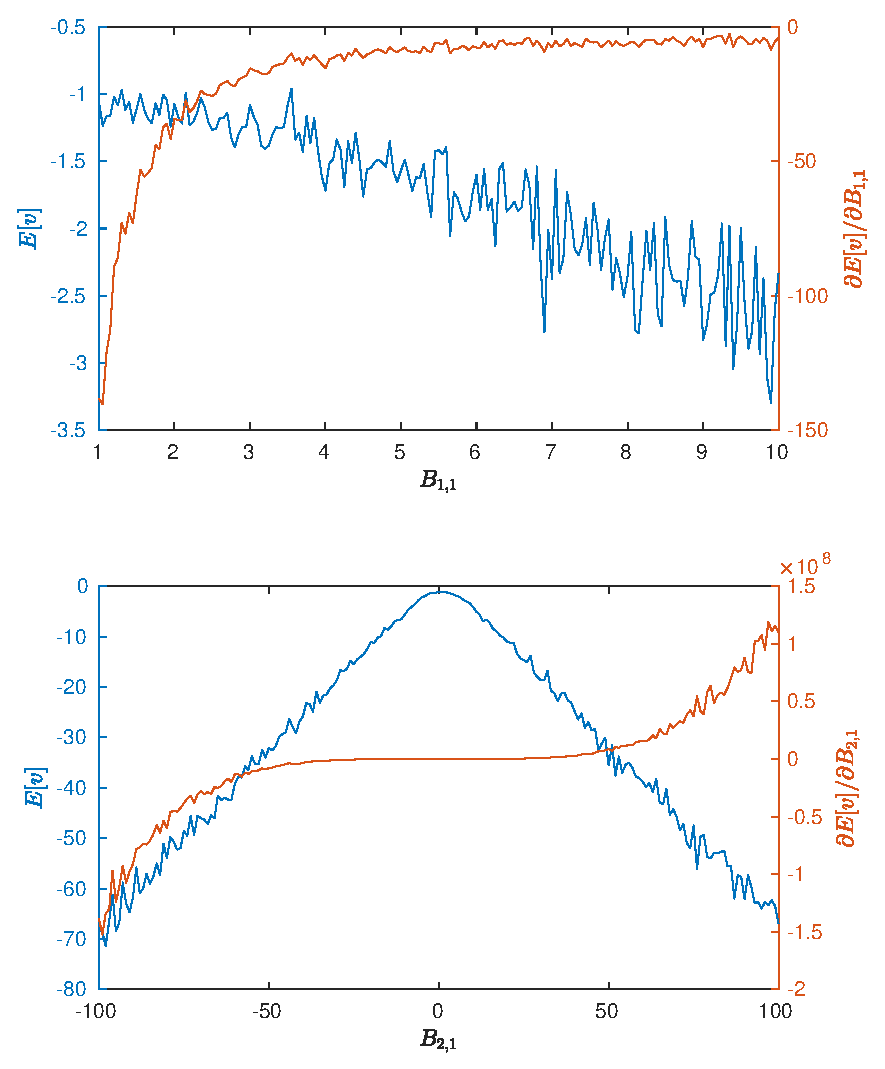
\includegraphics[width=0.8\columnwidth]{elbo_over_B_short}
  \end{minipage}
  \caption{How a well-defined problem with a correct solutions becomes a
    well-defined problem with an incorrect solution. In each plot, the function
    we are trying to optimise is in blue, and its derivative is in red. The
    plots on the left are for $q(\mathbf{u})$ and its derivatives with respect
    to $B_{1,1}$ (at the top) and $B_{2,1}$ (at the bottom), whereas the plots
    on the right are for $\mathbb{E}[v]$ and its corresponding derivatives.}
  \label{fig:B_gradient}
\end{figure*}

\begin{figure*}
  \centering
  \begin{minipage}{.5\textwidth}
    \centering
    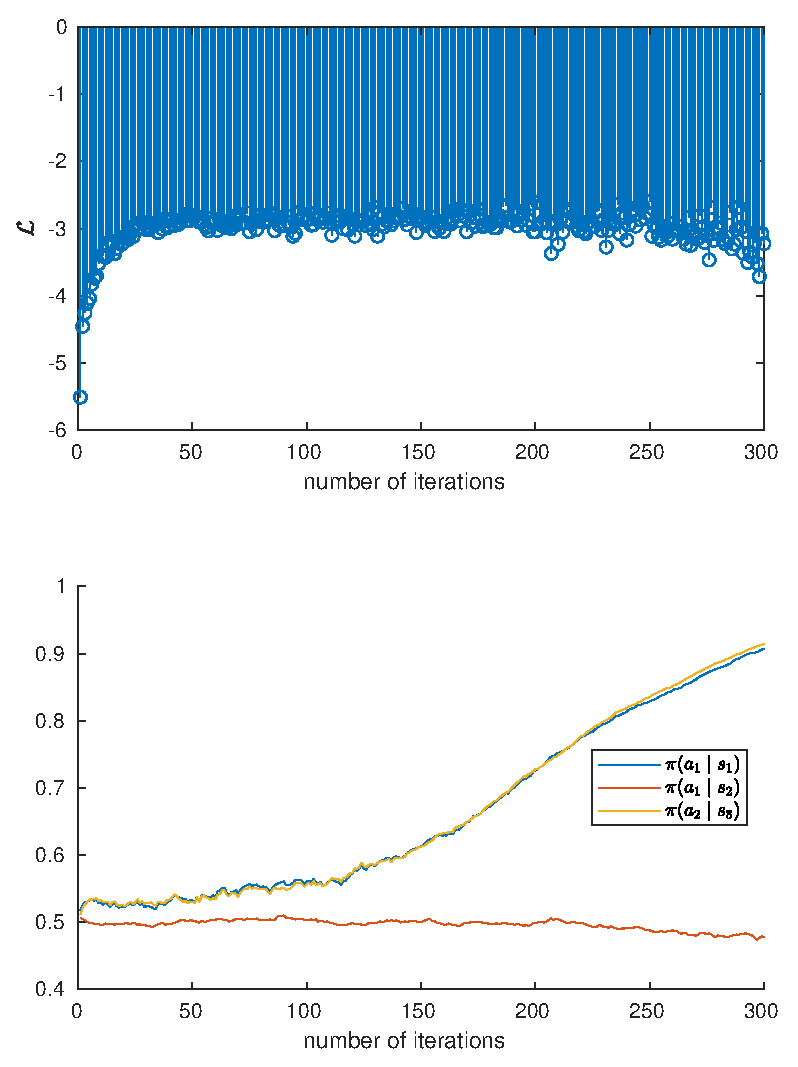
\includegraphics[width=0.8\columnwidth]{convergence1}
  \end{minipage}%
  \begin{minipage}{.5\textwidth}
    \centering
    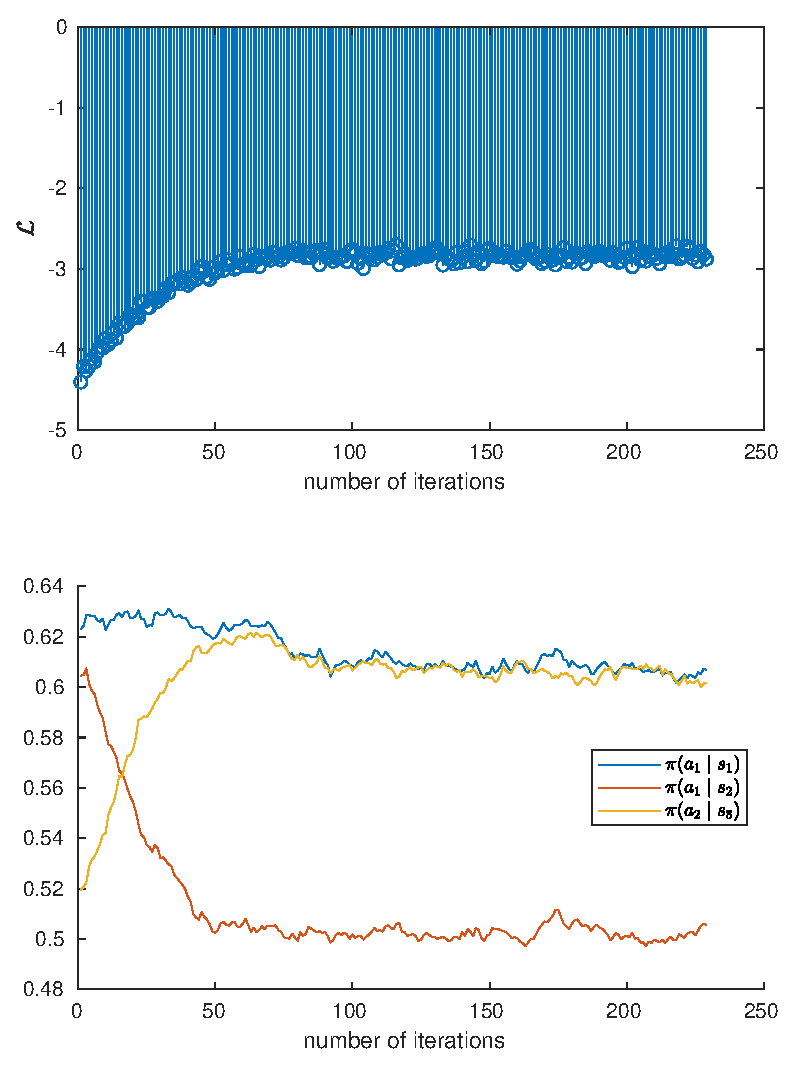
\includegraphics[width=0.8\columnwidth]{convergence2}
  \end{minipage}
  \caption{The convergence of $\mathcal{L}$ (at the top) and several example
    policies (at the bottom) over a number of iterations for Scenario~1 on the
    left and Scenario~2 on the right.}
  \label{fig:convergence1}
\end{figure*}

\begin{figure*}
  \centering
  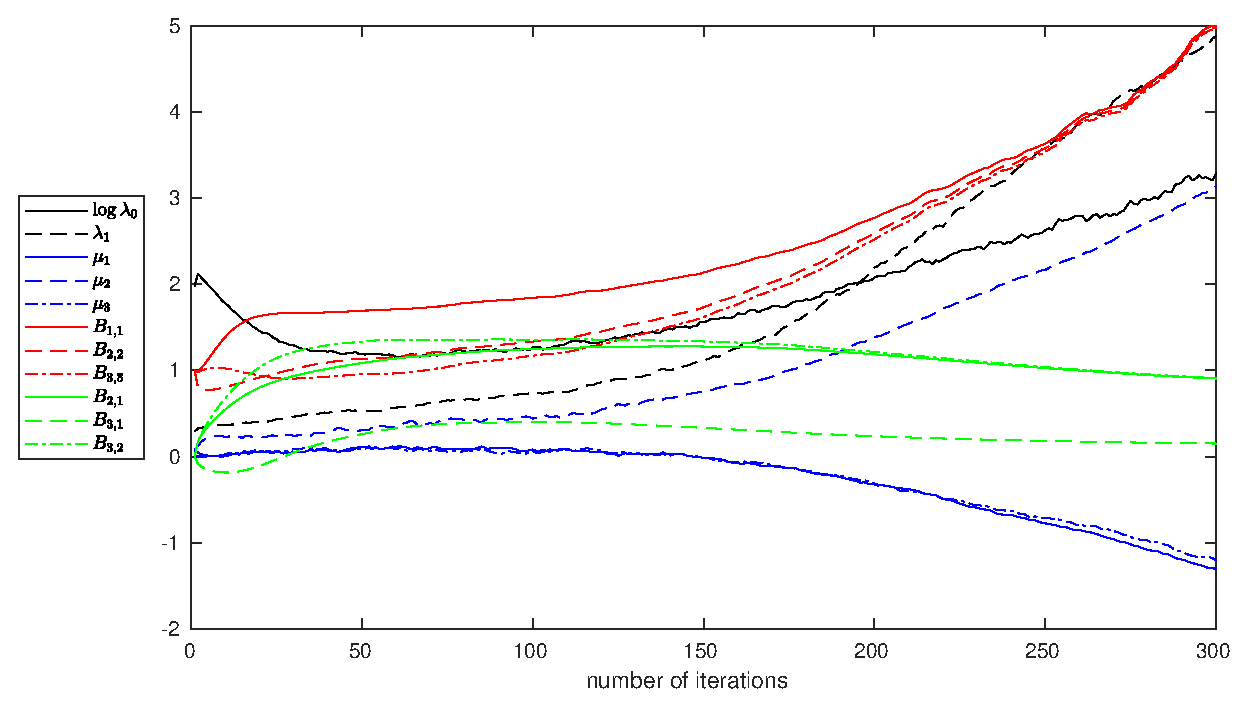
\includegraphics[width=\textwidth]{parameter_convergence1}
  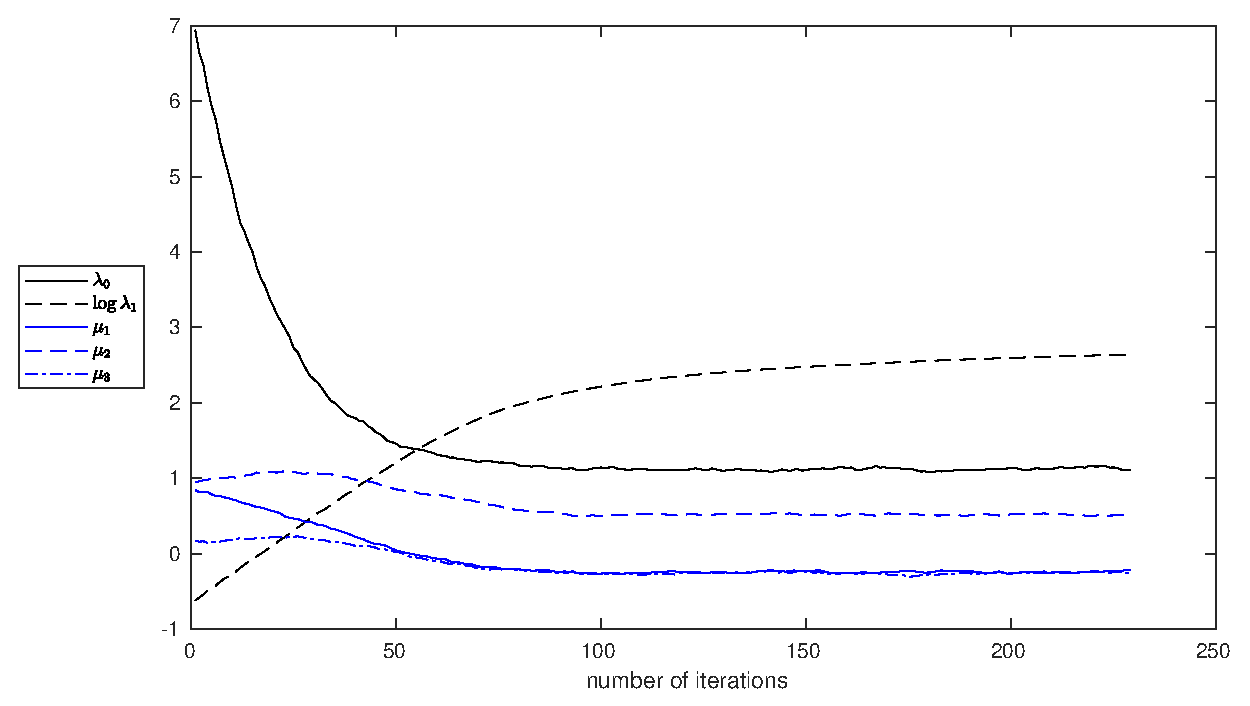
\includegraphics[width=\textwidth]{parameter_convergence2}
  \caption{Convergence of all optimised parameters for Scenario~1 at the top and
  Scenario~2 at the bottom. In order to represent different variables on the
  same scale, some variables have been $\log$-transformed. Colours denote which
  vector or matrix each scalar comes from: black for $\bm\lambda$,
  \textcolor{blue}{blue} for $\bm\mu$, \textcolor{red}{red} for diagonal
  elements of $\mathbf{B}$, and \textcolor{green}{green} for its non-diagonal
  elements.}
  \label{fig:convergence2}
\end{figure*}

Unfortunately, we are not able to use $\frac{\partial \mathcal{L}}{\partial
  \mathbf{B}}$ in order to optimise $\mathbf{B}$. We illustrate the problem in
Figure \ref{fig:B_gradient}. On the left side of the figure, we plot how
$q(\mathbf{u})$ behaves as a function of a diagonal and a non-diagonal element
of $\mathbf{B}$. Both functions have maximum values that can be attained by
following the corresponding derivatives. However, when these derivatives are
used to estimate $\frac{\partial \mathbb{E}[v]}{\partial \mathbf{B}}$, the
resulting derivatives no longer match their corresponding functions, although
the functions themselves still have optimal values: at or below $1$ for
$B_{1,1}$ and at $0$ for $B_{2,1}$. This leads us to consider two restrictions
of the model in order to investigate its convergence behaviour:
\begin{itemize}
\item In \textbf{Scenario 1}, we remove $\frac{\partial \mathbb{E}[v]}{\partial
    \mathbf{B}}$ from $\frac{\partial \mathcal{L}}{\partial \mathbf{B}}$. This
  essentially optimises $\mathbf{B}$ to match $\Kuu$, because then
  $\frac{\partial \mathcal{L}}{\partial \mathbf{B}}$ becomes
  $-\frac{\partial}{\partial \mathbf{B}} \DKL{q(\mathbf{u})}{p(\mathbf{u})}$,
  i.e., we are optimising $\mathbf{B}$ to minimise the difference between the
  prior and the posterior of $\mathbf{u}$.
\item In \textbf{Scenario 2}, we set $\mathbf{B} = \mathbf{I}_m$, and do not
  optimise it at all.
\end{itemize}

We plot how $\mathcal{L}$ as well as policies $\pi(a_1 \mid s_1)$, $\pi(a_2 \mid
s_3)$, and $\pi(a_1 \mid s_2)$ converge over a number of iterations in Figure
\ref{fig:convergence1}. The first two policies correspond to actions taken in
the set of demonstrations $\mathcal{D}$, so we would expect to see their
probabilities converge to values above $0.5$. Note that due to the stochastic
nature of our MDP model, we do not expect to see any probability reach exactly
$1$. The third policy, however, has no relevant data in $\mathcal{D}$, so the
maximum causal entropy framework would put the probability at around $0.5$.

As we ran the algorithm with two stopping conditions---$300$ iterations and the
$\ell_1$-norm of the change in parameter values being below $0.01$---note that
the algorithm terminated early in Scenario~2 but not in Scenario~1, although
there is clear convergence in both cases. An important difference is that
$\pi(a_1 \mid s_1)$ and $\pi(a_2 \mid s_3)$ converge closer and closer to $1$
with the slightly-restricted model of Scenario~1, but stabilise at $0.6$ in
Scenario~2 due to an important part of the model being completely fixed. In both
cases, $\pi(a_1 \mid s_2)$ converges to $0.5$ as expected.

Figure \ref{fig:convergence2} shows how the parameters of the model converge in
both scenarios. The algorithm seems to converge fine in Scenario~2, but most of
the parameters fail to stabilise in Scenario~1. Most importantly, the diagonal
values of the $\mathbf{B}$ matrix diverge to positive infinity, leading to higher
variance in ELBO estimates seen in Figure \ref{fig:convergence1}. The
non-diagonal values, however, converge just fine. Both $\lambda_0$ and
$\lambda_1$ also diverge to positive infinity, while the elements of $\bm\mu$
diverge, but in `the right' direction: as $\mu_2$ increases while $\mu_1$ and
$\mu_3$ decrease, the policies in Figure \ref{fig:convergence1} converge to
their optimal values.

This leaves us with two models: one that converges to reasonable-but-suboptimal
values, and one that diverges to infinite variance but also provides correct
policies.

\section{Related Work} % 0.5-1 page

The IRL problem itself was originally proposed by Russell in 1998
\cite{DBLP:conf/colt/Russell98}. Most of the early approaches had the
aforementioned reward linearity assumption. One of the first papers on the
subject by Ng and Russell \cite{DBLP:conf/icml/NgR00} introduced several linear
programming algorithms and identified an important issue: there are typically
many reward functions that can explain the data equally well. This problem was
solved by Ziebart et al. \cite{ziebart2008maximum} with the introduction of IRL
based on the principles of maximum causal entropy in a linearly-solvable MDP.

Levine et al. \cite{DBLP:conf/nips/LevinePK11} were the first to lift the
linearity assumption without imposing additional restrictions on the problem.
They do, however, model rewards as having no variance---our work removes this
restriction without any compromises.

Recently, Jin et al. \cite{DBLP:conf/uai/JinDAS17} have adapted the model
proposed by Levine et al. \cite{DBLP:conf/nips/LevinePK11} to use deep GPs,
harnessing the power of deep learning to make the model less dependent on what
features are provided. Although they use VI, their approximating distribution
for rewards at inducing points is simply the Dirac $\delta$ function, which is
essentially equivalent to the assumption of no variance.

An alternative to GPs for modelling nonlinear functions is, of course, neural
networks. Wulfmeier et al. \cite{wulfmeier2015maximum} have shown how they can
be used in the IRL setting. While this approach benefits from constant-time
inference and the ability to learn complex features from data, neural
networks often need significantly more data for the weights across all layers to
stabilise.

\subsection{Variational Inference}
% none of these approaches really work in our situation because they tend to
% depend on properties of how GPs are used in regression that are no longer true
% in IRL

Since the focus of our work was on proving feasibility rather than ensuring
performance, we simply used a combination of Gaussians for our variational
approximation. However, while VI was initially focused on approximating
distributions using simplistic models where all variables are independent
\cite{blei2017variational}, the last few years have brought many advances in
approximating more complex distributions and greatly reducing the computational
complexity of the task. Adapting some of them to IRL is a nontrivial but highly
valuable undertaking.

For approximating complex distributions, Rezende and Mohamed
\cite{DBLP:conf/icml/RezendeM15} suggest using \emph{normalising flows}, i.e., a
collection of invertible functions---parametrised by additional variational
parameters---that are applied to latent variables. A major challenge in applying
their work to IRL is related to variational parameters being used to compute the
MDP value function, i.e., how can we take the derivative of the value function
with respect to such a variational parameter? Alternatively, perhaps one can
construct a different model that would make this question moot.

Another approach to flexibility in modelling could come from considering
different GP kernels. For instance, Wilson and Adams \cite{pmlr-v28-wilson13}
show how all \emph{stationary} (i.e., invariant to translations) kernels can be
generated (or at least approximated) from a mixture of Gaussians in their
spectral representation using Bochner's theorem
\cite{bochner1959lectures,DBLP:journals/technometrics/Woodard00}. It looks
promising to combine these kernels with the variational Fourier features
approach by Hensman et al. \cite{DBLP:journals/jmlr/HensmanDS17} that leverages
the same spectral representations for efficient VI.

\section{Conclusions}
% TODO: write

% Show how we achieved our claimed contributions

Reasonable results in convergence.
More variables/information. Fewer assumptions.

We show how to avoid the deterministic training conditional assumption.

%Why doesn't it work? Perhaps a stupid bug.

\subsection{Further Work}

An interesting extension to our work would be to consider IRL in the context
of a reinforcement learning (RL) agent. Suppose we have an agent whose purpose
is to learn optimal behaviour from observing other agents using IRL. It could
then take reward variance estimates into account when choosing what states to
visit next. It would have to handle the balance between exploration and
exploitation similarly to many RL agents, but the information about rewards
would come from observing (presumably near-optimal) behaviour exhibited by other
agents rather than directly from the environment.

It is also worth noting the approach presented in this paper requires solving
$S$ MDPs for every iteration of optimising the parameters (where $S$ is the
number of samples drawn from $\approximation$). There are at least two ways to
reduce or eliminate this performance bottleneck:
\begin{itemize}
\item The MDP value function could be approximated, allowing for some minor
  mistakes in the resulting policy.
\item Perhaps there is a good way to use information about previously computed
  value functions for similar rewards to hasten the current computation. One
  simple way to do this would be by initialising the current values to the
  optimal values of the previous MDP value function computation.
\end{itemize}

Finally, building on the idea that variance estimates can be used to judge
whether the model has learned optimal policy, an interesting question for
MDP (or, perhaps, dynamical systems) research would be: how much does a reward
have to change in order to affect the deterministic policy? A simple answer to
this question would allow us to use variance estimates in order to quantify the
model's confidence regarding optimal behaviour.

%\vskip8pt \noindent
%{\bf Acknowledgments.}
%This is optional; it is a location for you to thank people
\bibliographystyle{abbrv}
\bibliography{paper}

\appendix
\section{Proofs} \label{appendix:proofs}

\derivatives*
\begin{proof}
  \leavevmode
  \begin{enumerate}
  \item
    \[
      \begin{split}
        \frac{\partial q(\mathbf{u})}{\partial m} &=
        q(\mathbf{u})\dm\left[-\frac{Q}{2}\right]
        \\
        &= -\frac{1}{2}q(\mathbf{u})(\bm\Sigma^{-1} +
        \bm\Sigma^{-\intercal})(\mathbf{u} - \bm\mu)\dm[\mathbf{u} -
        \bm\mu] \\
        &= \frac{1}{2}q(\mathbf{u})(\bm\Sigma^{-1} +
        \bm\Sigma^{-\intercal})(\mathbf{u} - \bm\mu).
      \end{split}
    \]
  \item An online tool by Laue et
    al.\footnote{\url{http://www.matrixcalculus.org/}}
    \cite{DBLP:conf/nips/LaueMG18} can be used to find both derivatives.
  \item
    \begin{enumerate}
    \item Since
    \begin{align*}
      q(\mathbf{r} \mid \mathbf{u}) &= \mathcal{N}(\mathbf{r};
      \Kru^\intercal\Kuu^{-1}\mathbf{u}, \Krr - \Kru^\intercal \Kuu^{-1}\Kru) \\
      &= \mathcal{N}(\mathbf{r}; \mathbf{Su}, \bm\Gamma),
    \end{align*}
    we have
    \[
      \frac{\partial q(\mathbf{r} \mid \mathbf{u})}{\partial \lambda_i} =
      -\frac{1}{2}q(\mathbf{r} \mid \mathbf{u}) \dl[(\mathbf{r} -
      \mathbf{Su})^\intercal\bm\Gamma^{-1}(\mathbf{r} - \mathbf{Su}) +
      \log|\bm\Gamma|].
    \]
    The same online tool can be used to show that
    \[
      \dl \log|\bm\Gamma| = -|\bm\Gamma|^{-1}\tr(\mathbf{R}\adj(\bm\Gamma)),
    \]
    and
    \[
      \dl \bm\Gamma^{-1} = \bm\Gamma^{-1}\mathbf{R}\bm\Gamma^{-1}.
    \]
  \item
    If $i=0$, then
    \[
      \frac{\partial \mathbf{K}}{\partial \lambda_i} =
      \frac{1}{\lambda_i}\mathbf{K}
    \]
    by the structure of each element of $\mathbf{K}$. If $i \ne 0$, then each
    element of $\frac{\partial \mathbf{K}}{\partial \lambda_i}$ is
    \begin{align*}
      L_{j,k} &= \frac{\partial k(\mathbf{x}_j, \mathbf{x}_k)}{\partial \lambda_i} \\
      &\begin{aligned}
        = k(\mathbf{x}_j, \mathbf{x}_k) \dl \left[ \vphantom{\frac{1}{2}} \right. &-\frac{1}{2}(\mathbf{x}_j - \mathbf{x}_k)^\intercal \bm\Lambda (\mathbf{x}_j - \mathbf{x}_k) \\
        &- \mathbbm{1}[j \ne k]\sigma^2\tr(\bm\Lambda) \left. \vphantom{\frac{1}{2}} \right]
      \end{aligned} \\
      &\begin{aligned}
        = k(\mathbf{x}_j, \mathbf{x}_k) \dl \left[ \vphantom{\sum_{k=1}^d} \right. &-\frac{1}{2} \sum_{l=1}^d \lambda_l (x_{j,l} - x_{k,l})^2 \\
        &- \mathbbm{1}[j \ne k]\sigma^2\sum_{l=1}^d \lambda_l \left. \vphantom{\sum_{l=1}^d} \right]
      \end{aligned} \\
      &= k(\mathbf{x}_j, \mathbf{x}_k) \left( -\frac{1}{2}(x_{j,i} - x_{k,i})^2 - \mathbbm{1}[j \ne k]\sigma^2 \right).
    \end{align*}
    \end{enumerate}
  \end{enumerate}
\end{proof}

\section{Derivatives of the ELBO}

\subsection{\texorpdfstring{$\partial/\partial\bm\mu$}{Derivative w.r.t. mu}}

We begin by removing terms independent of $\bm\mu$:
\[
  \frac{\partial\mathcal{L}}{\partial\bm\mu} =
  \dm[\mathbf{t}^\intercal\Kru^\intercal\Kuu^{-1}\bm\mu] - \frac{1}{2} \dm
  \left[ \bm\mu^\intercal \Kuu^{-1} \bm\mu \right] - \dm\mathbb{E}[v].
\]
Here
\[
  \dm \left[ \bm\mu^\intercal \Kuu^{-1} \bm\mu \right] = (\Kuu^{-1} +
  \Kuu^{-\intercal}) \bm\mu
\]
by Petersen and Pedersen \cite{petersen2008matrix}, and
\[
  \begin{split}
    \dm\mathbb{E}[\V(s)] &= \dm\iint \V(s) q(\mathbf{r} \mid \mathbf{u})
    q(\mathbf{u})\dx \\
    &= \iint \V(s) q(\mathbf{r} \mid \mathbf{u}) \frac{\partial
      q(\mathbf{u})}{\partial \bm\mu}\dx \\
    &= \frac{1}{2}\mathbb{E}[\V(s) (\bm\Sigma^{-1} +
    \bm\Sigma^{-\intercal})(\mathbf{u} - \bm\mu)]
  \end{split}
\]
by Theorem \ref{thm:main} and Lemma \ref{lemma:derivatives}. Hence,
\[
  \begin{split}
    \frac{\partial\mathcal{L}}{\partial\bm\mu} &=
    \mathbf{t}^\intercal\Kru^\intercal\Kuu^{-1} - \frac{1}{2} (\Kuu^{-1} +
    \Kuu^{-\intercal}) \bm\mu \\
    &- \frac{1}{2}\mathbb{E} \left[(\bm\Sigma^{-1} +
      \bm\Sigma^{-\intercal})(\mathbf{u} - \bm\mu) v \right].
  \end{split}
\]

\subsection{\texorpdfstring{$\partial/\partial\mathbf{B}$}{Derivative w.r.t. B}}

\[
  \frac{\partial\mathcal{L}}{\partial\mathbf{B}} =
  \frac{1}{2} \left( \dB\log|\bm\Sigma| - \dB\tr \left( \Kuu^{-1} \bm\Sigma
    \right) \right)
  - \dB\mathbb{E}[v].
\]
By Theorem \ref{thm:main},
\[
  \dB\mathbb{E}[\V(s)] = \iint \V(s) q(\mathbf{r} \mid \mathbf{u})
  \frac{\partial q(\mathbf{u})}{\partial \mathbf{B}}\dx.
\]
Then, using the aforementioned tool by Laue et al.
\cite{DBLP:conf/nips/LaueMG18}, we get
\[
  \dB\log|\bm\Sigma| = 2\bm\Sigma^{-1}\mathbf{B}, \quad \dB \tr \left( \Kuu^{-1}
    \bm\Sigma \right) = 2\Kuu^{-1}\mathbf{B},
\]
and Lemma \ref{lemma:derivatives} gives
\begin{gather*}
  \frac{\partial q(\mathbf{u})}{\partial \mathbf{B}} =
  q(\mathbf{u})(\bm\Sigma^{-1}\mathbf{U}\bm\Sigma^{-1} -
  |\bm\Sigma|^{-1}\adj(\bm\Sigma))\mathbf{B}.
\end{gather*}
Therefore,
\begin{gather*}
  \frac{\partial \mathcal{L}}{\partial \mathbf{B}} =
  \left( \bm\Sigma^{-1} - \Kuu^{-1} \right) \mathbf{B} - \mathbb{E}
  [(\bm\Sigma^{-1}\mathbf{U}\bm\Sigma^{-1} -
  |\bm\Sigma|^{-1}\adj(\bm\Sigma))\mathbf{B}v].
\end{gather*}

\subsection{\texorpdfstring{$\partial/\partial \lambda_j$}{Derivative w.r.t.
    Lambda}}

For $j = 0, \dots, d$,
\[
  \begin{split}
    \frac{\partial \mathcal{L}}{\partial \lambda_j} &= \mathbf{t}^\intercal\dlj
    \left[ \Kru^\intercal\Kuu^{-1} \right] \bm\mu - \dlj\mathbb{E}[v] \\
    &- \frac{1}{2} \left(\dlj \tr \left(\Kuu^{-1}\bm\Sigma \right) +
      \bm\mu^\intercal \frac{\partial \Kuu^{-1}}{\partial \lambda_j} \bm\mu +
      \dlj \log |\Kuu| \right),
  \end{split}
\]
where
\begin{align*}
  \frac{\partial \Kuu^{-1}}{\partial \lambda_j} &= -\Kuu^{-1}\frac{\partial \Kuu}{\partial \lambda_j}\Kuu^{-1}, \\
  \dlj \left[ \Kru^\intercal\Kuu^{-1} \right] &= \frac{\partial \Kru^\intercal}{\partial \lambda_j} \Kuu^{-1} + \Kru^\intercal \frac{\partial \Kuu^{-1}}{\partial \lambda_j} \\
                                                &= \left( \frac{\partial \Kru^\intercal}{\partial \lambda_j} - \Kru^\intercal\Kuu^{-1}\frac{\partial \Kuu}{\partial \lambda_j} \right) \Kuu^{-1}, \\
  \dlj \tr(\Kuu^{-1}\bm\Sigma) &= \tr \left( \dlj \left[ \Kuu^{-1}\bm\Sigma \right] \right) = \tr \left( \frac{\partial \Kuu^{-1}}{\partial \lambda_j} \bm\Sigma \right) \\
                                                &= -\tr \left( \Kuu^{-1} \frac{\partial \Kuu}{\partial \lambda_j} \Kuu^{-1} \bm\Sigma \right), \\
  \dlj\log|\Kuu| &= \tr \left( \Kuu^{-1} \frac{\partial \Kuu}{\partial \lambda_j} \right)
\end{align*}
by Petersen and Pedersen \cite{petersen2008matrix}, and
\[
  \begin{split}
    \dlj \mathbb{E}[\V(s)] &= \iint\V(s)\frac{\partial q(\mathbf{r} \mid
      \mathbf{u})}{\partial \lambda_j}q(\mathbf{u})\dx \\
    &= \!\begin{multlined}[t]
      \frac{1}{2}\mathbb{E}[\V(s) (|\bm\Gamma|^{-1} \tr(\mathbf{R}
          \adj(\bm\Gamma)) \\
          - (\mathbf{r} -
          \mathbf{Su})^\intercal\bm\Gamma^{-1}\mathbf{R}\bm\Gamma^{-1}(\mathbf{r}
          - \mathbf{Su}))]
    \end{multlined}
  \end{split}
\]
by Theorem \ref{thm:main} and Lemma \ref{lemma:derivatives}. Thus,
\begin{align*}
  \frac{\partial \mathcal{L}}{\partial \lambda_j} &=
  \mathbf{t}^\intercal \left( \frac{\partial \Kru^\intercal}{\partial
      \lambda_j} - \Kru^\intercal\Kuu^{-1}\frac{\partial
      \Kuu}{\partial \lambda_j} \right) \Kuu^{-1} \bm\mu \\
  &\begin{aligned}
    + \frac{1}{2} \left[ \vphantom{\frac{\partial \Kuu}{\partial \lambda_j}}
    \right. &\tr \left( \Kuu^{-1} \frac{\partial \Kuu}{\partial \lambda_j}
      \Kuu^{-1} \bm\Sigma \right) + \bm\mu^\intercal \Kuu^{-1} \frac{\partial
      \Kuu}{\partial \lambda_j} \Kuu^{-1} \bm\mu \\
    &- \tr \left. \left(\Kuu^{-1} \frac{\partial \Kuu}{\partial \lambda_j}
      \right) \right]
  \end{aligned} \\
  &\begin{aligned}
    - \frac{1}{2} \mathbb{E} [ (&|\bm\Gamma|^{-1} \tr(\mathbf{R} \adj(\bm\Gamma)) \\
    &- (\mathbf{r} - \mathbf{Su})^\intercal\bm\Gamma^{-1}\mathbf{R}\bm\Gamma^{-1}(\mathbf{r} - \mathbf{Su})) v],
  \end{aligned} 
\end{align*}
where the remaining derivatives can be found in Lemma \ref{lemma:derivatives}.

\end{document}